\clearpage
\thispagestyle{empty}
\null
\newpage

\cleardoublepage
\phantomsection
% \pdfbookmark[1]{Etat de l'art}{Etat de l'art}
% \addcontentsline{toc}{part}{Etat de l'art}
\markboth{\spacedlowsmallcaps{Etat de l'art}}{\spacedlowsmallcaps{Etat de l'art}}
\part{Etat de l'art}
\label{part:etat_art}

\clearpage
\thispagestyle{empty}
\null
\newpage

% \acn{TODO}:
%  - Globalement, harmoniser le vocabulaire
%  - Globalement, introduire correctement les termes techniques/théoriques comme "Adéquation organisationel", "\acn{RNN}", "\acn{VAE}", "\acn{LSTM}", "World Models" notamment pour permettre à un lecteur non familier avec le \acn{ML} ou l'\acn{IA} en général de comprendre.
%  - Reformater pour mettre en valeur le sous-problème accompagné de l'hypothèse associé, puis établir un état de l'art dans l'espace de recherche délimité par l'hypothèse afin de répondre au sous-problème : donner un aperçu de l'état de l'art avec une synthèse sous forme de table qui permet de voir comment les travaux (appartenant à cet espace de recherche délimité par l'hypothèse) permettent de répondre au mieux au sous-problèmes (c'est à dire comment un travail permet de couvrir les objectifs d'un sous-problème). Cela permet aussi de voir les objectifs des sous-problèmes qui sont bien couverts dans la littérature, moyennement couvert ou pas du tout couvert. Donc à la fin, on peut déterminer les travaux qui couvre le plus d'objectifs d'un sous-problème mais aussi les objectifs encore non-couverts présentés sous la forme de verrous théoriques ou techniques.
%  - A la fin on doit donc savoir quels sont les travaux les plus prometteurs et les verrous restants qui restent à relever par des contributions qui seront présentées dans la partie suivante sur la méthode

\chapter*{Introduction}
\addcontentsline{toc}{chapter}{\textbf{Introduction}}

\noindent
Cette partie vise à identifier et analyser les approches les plus pertinentes pour résoudre les quatre sous-problèmes issus de la décomposition du problème de conception d'un \acn{SMA} de Cyberdéfense, formalisé comme un problème d'optimisation sous contraintes. L'objectif est de recenser les travaux permettant de répondre aux critères spécifiques de chaque sous-problème, tout en mettant en lumière les verrous scientifiques et techniques qui subsistent, afin de capitaliser au mieux sur les avancées existantes.

Le premier chapitre propose une revue critique de la littérature pour chacun des sous-problèmes, en s'appuyant sur les quatre grandes activités de la démarche. Il s'agit d'identifier, pour chaque activité, les contributions majeures susceptibles de satisfaire les critères fixés, ainsi que les principaux verrous qui justifient la nécessité de nouvelles avancées méthodologiques.

Le second chapitre approfondit l'étude des travaux identifiés comme les plus prometteurs, afin de fournir un socle théorique solide pour expliquer et circonscrire techniquement les verrous identifiés. Ce chapitre introduit ainsi les concepts fondamentaux qui serviront de base aux futures contributions méthodologiques de la méthode proposée.

La \autoref{fig:organisation_manuscrit_partie_2} synthétise l'organisation de cette partie et les liens logiques entre chapitres et sous-sections.


\begin{figure}[h!]
  \centering
  \resizebox{0.8\textwidth}{!}{%
    \begin{tikzpicture}[
    chapter/.style={draw, fill=blue!10, thick, minimum width=8cm, minimum height=1.2cm, text centered, font=\bfseries},
    section/.style={draw, fill=blue!5, thick, minimum width=7cm, minimum height=1cm, text centered, font=\small},
    arrow/.style={-Latex, thick},
    node distance=0.4cm,
    annotated/.style={above,font=\small\itshape, inner sep=1pt, yshift=0.8cm, xshift=-7cm}
]

% Chapitre 4
\node[chapter] (ch4) {\parbox{10cm}{Chapitre 4 : Les SMA et concepts théoriques mobilisés}};

\node[section, below=1cm of ch4, xshift=-1cm] (ch4s1) {\parbox{8cm}{SMA et modèles organisationnels}};
\node[section, below=1cm of ch4s1] (ch4s2) {\parbox{8cm}{Apprentissage par renforcement multi-agent}};
\node[section, below=1cm of ch4s2] (ch4s3) {\parbox{8cm}{Modéliser un environnement simulé : les techniques \textquote{World Models}}};

\draw[arrow] ($ (ch4.south) + (4.0,0) $) -- ++(0,0) |- (ch4s1.east) node[annotated] {Les bases du raisonnement organisationnel sont introduites pour structurer le comportement des SMA.};
\draw[arrow] ($ (ch4.south) + (4.0,0) $) -- ++(0,0) |- (ch4s2.east) node[annotated] {Ce cadre organisationnel doit être articulé avec les techniques d’apprentissage multi-agent.};
\draw[arrow] ($ (ch4.south) + (4.0,0) $) -- ++(0,0) |- (ch4s3.east) node[annotated] {L’apprentissage nécessite un environnement simulé, souvent construit par des World Models.};


% Chapitre 5
\node[chapter, below=1cm of ch4s3, xshift=1cm] (ch5) {\parbox{10cm}{Chapitre 5 : Revue de littérature, analyse et verrous liés aux hypothèses}};

\node[section, below=1cm of ch5, xshift=-1cm] (ch5s1) {\parbox{8cm}{Un cadre Markovien pour formaliser le problème \\ de conception et sa résolution en MARL (H1)}};
\node[section, below=1cm of ch5s1] (ch5s2) {\parbox{8cm}{Les Worlds Models pour simuler des \\ environnement multi-agents (H2)}};
\node[section, below=1cm of ch5s2] (ch5s3) {\parbox{8cm}{L'intégration de contraintes/guidages \\ organisationnelles dans le processus MARL (H3)}};
\node[section, below=1cm of ch5s3] (ch5s4) {\parbox{8cm}{L'extraction automatisée des spécifications \\ organisationnelles émergentes (H4)}};

\draw[arrow] ($ (ch4.south) + (4.5,0) $) -- ($ (ch5.north) + (4.5,0) $) node[annotated, yshift=-0.5cm] {À partir de ces concepts, chaque hypothèse est examinée à travers une revue ciblée.};

\draw[arrow] ($ (ch5.south) + (4.0,0) $) -- ++(0,0) |- (ch5s1.east) node[annotated] {La première étape consiste à formuler formellement le problème de conception.};
\draw[arrow] ($ (ch5.south) + (4.0,0) $) -- ++(0,0) |- (ch5s2.east) node[annotated] {Cela suppose la disponibilité d’un environnement simulé fidèle aux dynamiques réelles.};
\draw[arrow] ($ (ch5.south) + (4.0,0) $) -- ++(0,0) |- (ch5s3.east) node[annotated] {Dans ce cadre simulé, l’apprentissage doit être guidé par des contraintes organisationnelles.};
\draw[arrow] ($ (ch5.south) + (4.0,0) $) -- ++(0,0) |- (ch5s4.east) node[annotated] {Enfin, les comportements appris doivent pouvoir être interprétés sous forme de structures émergentes.};

\end{tikzpicture}

  }
  \caption{Structure de la Partie II~: Etat de l'art}
  \label{fig:organisation_manuscrit_partie_2}
\end{figure}

\clearpage
\thispagestyle{empty}
\null
\newpage


\chapter{Les verrous d'une méthode de conception}
\label{chap:verrous}

\noindent
Ce chapitre a pour objectif d'introduire et d'analyser les principaux verrous scientifiques liés à la conception automatisée de \acplu{SMA}, tels qu'ils émergent de la décomposition du problème en quatre grandes activités : modélisation, résolution, analyse et transfert. Pour chacune de ces activités, un sous-problème fondamental (\textbf{MOD} à \textbf{TRF}) a été identifié, associé à une hypothèse de restriction de l'espace de recherche (\textbf{H-MOD} à \textbf{H-TRF}). Nous définissons pour chaque sous-problème un ensemble de critères spécifiques permettant d'évaluer la couverture des approches existantes. La revue de littérature conduite selon ces critères permet de cartographier les travaux les plus pertinents, d'identifier les avancées majeures, ainsi que les verrous et lacunes qui subsistent. Ce chapitre propose ainsi une analyse critique de l'état de l'art pour chaque hypothèse, en vue de dégager les défis à relever et de motiver les contributions méthodologiques présentées dans la suite du manuscrit.

\section{La modélisation d'un environnement en simulation (H-MOD)}

\subsection*{Recontextualisation du sous-problème dans la démarche de la thèse}

Le premier sous-problème fondamental identifié dans notre approche concerne la \textbf{modélisation réaliste de l'environnement} (\textbf{MOD}). Cette étape est cruciale car elle conditionne la crédibilité des expérimentations, l'entraînement des agents et, in fine, la validité des politiques de Cyberdéfense obtenues. Dans le cadre de la thèse, la simulation d'un environnement pertinent permet de tester, d'évaluer et d'optimiser les comportements multi-agents sans exposer de systèmes réels à des risques opérationnels. Elle constitue ainsi le socle expérimental sur lequel reposent les phases ultérieures d'apprentissage, d'analyse et de transfert. \subsection*{Objectif global et critères spécifiques} L'objectif principal de cette activité est d'obtenir un environnement simulé qui soit à la fois \textbf{réaliste}, \textbf{adaptable}, \textbf{fidèle aux dynamiques du monde réel} et \textbf{exploitables pour l'entraînement et l'évaluation des agents}. Pour guider la revue de littérature, nous retenons les critères spécifiques suivants :
%
\begin{itemize}
  \item \textbf{Fidélité} : capacité à reproduire les dynamiques, menaces et interactions observées dans des environnements réels ; \emph{ce critère est essentiel pour garantir que les politiques apprises en simulation soient pertinentes et transférables au monde réel}.
  \item \textbf{Adaptabilité} : possibilité de modifier facilement la topologie, les scénarios ou les paramètres pour explorer différents contextes ; \emph{cela permet de tester la robustesse des agents face à des environnements variés et d'étudier des cas d'usage multiples}.
  \item \textbf{Automatisation} : degré d'automatisation de la génération ou de l'évolution de l'environnement simulé ; \emph{une automatisation élevée facilite la création rapide de nouveaux scénarios et réduit la dépendance à l'expertise humaine}.
  \item \textbf{Interopérabilité} : aptitude à intégrer ou à échanger des données avec d'autres outils ou plateformes ; \emph{ce critère favorise la réutilisation, la comparaison et l'intégration de résultats issus de différents systèmes ou sources de données}.
  \item \textbf{Facilité d'utilisation} : accessibilité pour les concepteurs, possibilité de personnalisation sans expertise avancée ; \emph{une utilisation aisée accélère le prototypage et démocratise l'expérimentation auprès d'utilisateurs non spécialistes}.
  \item \textbf{Multi-agent} : capacité de l'environnement à accueillir un ou plusieurs agents, et à gérer leurs interactions ; \emph{ce critère est indispensable pour étudier des scénarios collaboratifs ou compétitifs, et pour évaluer des approches multi-agents}.
\end{itemize}

\subsection*{Hypothèse de restriction de l'espace de recherche (\textbf{H-MOD})}

Afin de circonscrire l'espace de recherche à un domaine pertinent et exploitable, nous posons l'hypothèse suivante~: \textit{Il est possible d'obtenir un environnement simulé réaliste, soit en facilitant la modélisation manuelle, soit par des techniques d'apprentissage machine à partir de données}. Cette hypothèse nous conduit à concentrer la revue de littérature sur deux grandes familles de travaux~:

\begin{itemize}
  \item \textbf{La modélisation manuelle}~: regroupe tous les travaux où la création de l'environnement simulé repose sur une intervention humaine. Cela inclut les simulateurs (\acn{CybORG}, \acn{NASimEmu}, \acn{CYST}) et modèles d'environnements de Cyberdéfense génériques, dans lesquels la structure, les règles et les scénarios sont explicitement définis, totalement ou partiellement, par des experts. Cette approche permet de réutiliser des modèles existants, soit directement si l'environnement simulé correspond à l'environnement réel cible, soit après adaptation et instanciation du modèle de simulation générique. Bien que largement répandue, cette méthode limite souvent la généricité, car peu de modèles sont à la fois faciles à adapter et applicables à une grande diversité d'environnements de Cyberdéfense. On y retrouve également les formalismes Markoviens (\acn{MDP}, \acn{POMDP}, \acn{Dec-POMDP}, \acn{POSG}), qui servent de base théorique et pratique à la plupart des modélisations manuelles.
  \item \textbf{La modélisation basée sur l'apprentissage}~: regroupe les approches où la dynamique de l'environnement est apprise automatiquement à partir de données collectées dans l'environnement réel ou issues d'interactions. Cela inclut les travaux d'identification de systèmes (\textit{System Identification}), de modélisation de substitution (\textit{Surrogate Modeling}) ou de simulation guidée par les données (\textit{Data-Driven Simulation}).
\end{itemize}

Ce choix est motivé par l'état de l'art, qui montre que ces deux axes concentrent l'essentiel des avancées récentes et offrent des compromis différents entre fidélité, automatisation et adaptabilité.

\subsection*{Couverture des critères par les travaux identifiés}

Une synthèse de la couverture des critères par les travaux identifiés dans les sujets évoqués dans l'hypothèse (\textbf{H-MOD}) est présentée dans le \autoref{tab:couverture_criteres_travaux}.

\begin{table}[h!]
  \centering
  \caption{Couverture des critères spécifiques par les principales familles de travaux de modélisation d'environnements de Cyberdéfense}
  \label{tab:couverture_criteres_travaux}
  \tiny
  \renewcommand{\arraystretch}{1.4}
  \begin{tabularx}{\textwidth}{
      >{\raggedright\arraybackslash\hsize=0.4\hsize}X
      >{\raggedright\arraybackslash\hsize=0.1\hsize}X
      >{\raggedright\arraybackslash\hsize=0.1\hsize}X
      >{\raggedright\arraybackslash\hsize=0.1\hsize}X
      >{\raggedright\arraybackslash\hsize=0.1\hsize}X
      >{\raggedright\arraybackslash\hsize=0.1\hsize}X
      >{\raggedright\arraybackslash\hsize=0.1\hsize}X
    }
    \hline
    \textbf{Travaux / Critères}                                                                                                                            & \textbf{Fidélité} & \textbf{Adaptabilité} & \textbf{Automatisation} & \textbf{Interopérabilité} & \textbf{Facilité d'utilisation} & \textbf{Multi-agent} \\
    \hline
    Modèles formels génériques (\acn{MDP}, \acn{POMDP}, \acn{Dec-POMDP}, \acn{POSG}, graphes d'attaque, arbres \acn{AD}, réseaux de Petri, modèles de jeu) & \cmark{}          & \cmark{}              & \xmark{}                & \cmark{}                  & \xmark{}                        & \cmark{}             \\
    Frameworks génériques et configurables (\acn{CyberBattleSim}, \acn{NASim}, \acn{NASimEmu}, \acn{DETERLab}, \acn{CyberVAN}, \acn{CYST})                 & \cmark{}          & \cmark{}              & \xmark{}                & \cmark{}                  & \cmark{}                        & \cmark{}             \\
    Simulateurs spécialisés de Cyberdéfense (\acn{CybORG}, \acn{CybORG}++, CyberWheel, \acn{SCYTHE}, \acn{CTF})                                            & \cmark{}          & \xmark{}              & \xmark{}                & \cmark{}                  & \cmark{}                        & \cmark{}             \\
    System Identification                                                                                                                                  & \cmark{}          & \cmark{}              & \cmark{}                & \xmark{}                  & \xmark{}                        & \cmark{}             \\
    Surrogate Modeling                                                                                                                                     & \cmark{}          & \cmark{}              & \cmark{}                & \xmark{}                  & \cmark{}                        & \cmark{}             \\
    Data-Driven Simulation (World Models, simulation guidée par les données)                                                                               & \cmark{}          & \cmark{}              & \cmark{}                & \xmark{}                  & \xmark{}                        & \cmark{}             \\
    \hline
  \end{tabularx}
\end{table}

Concernant l'approche de modélisation manuelle, les travaux identifiés sont :

\paragraph{Les modèles formels génériques.}
Au niveau le plus abstrait, la modélisation des environnements de Cyberdéfense repose sur des formalismes mathématiques issus de la théorie de la décision séquentielle. Le cadre de base est le \textit{Markov Decision Process} (\acn{MDP})~\cite{puterman1994mdp}, qui décrit un environnement comme un ensemble d'états, d'actions et de transitions probabilistes. Lorsque l'information disponible est partielle, les \acn{POMDP}~\cite{kaelbling1998pomdp} offrent un cadre adapté. Pour les \acplu{SMA} coopératifs, les variantes décentralisées (\acn{Dec-POMDP})~\cite{Oliehoek2016} sont utilisées, tandis que les environnements compétitifs (attaquant/défenseur) sont modélisés par les \textit{Partially Observable Stochastic Games} (\acn{POSG})~\cite{hansen2004posg}. D'autres extensions, comme les \acn{MDP} factorisés~\cite{guestrin2003factored}, facilitent la modélisation de systèmes complexes, et la théorie des jeux de sécurité~\cite{manshaei2013game} permet de formaliser explicitement les stratégies adversariales.
Ces formalismes constituent la base théorique commune à la plupart des simulateurs et frameworks de cybersécurité. À côté des modèles markoviens, des représentations graphiques intermédiaires sont également utilisées. Les \textit{graphes d'attaque}~\cite{CPhilips1998} décrivent les différentes voies d'exploitation des vulnérabilités d'un réseau, tandis que les \textit{arbres attaque-défense}~\cite{BKordy2010} intègrent explicitement les contre-mesures défensives. Les \textit{réseaux de Petri}~\cite{MPetty2022,JBland2020,SYamaguchi2020} permettent de représenter et d'analyser des stratégies concurrentes d'attaque et de défense. Enfin, les \textit{modèles de jeu} appliqués à la cybersécurité~\cite{MPanfili2018,AAttiah2018,CXiaolin2008} formalisent les interactions attaquant/défenseur comme des jeux dynamiques, souvent non coopératifs, et constituent une passerelle naturelle vers les cadres \acn{POSG} et \acn{Dec-POMDP}~\cite{beynier2010,terry2020pettingzoo,bernstein2013}.
En résumé, ces modèles formels et graphiques offrent une boîte à outils générique et flexible pour construire des environnements de simulation adaptés à une grande variété de scénarios de cybersécurité.

\paragraph{Les frameworks génériques et configurables.}
Entre les formalismes abstraits et les simulateurs spécialisés, la littérature met en avant plusieurs frameworks visant à offrir un compromis entre généricité et exploitabilité. Parmi ceux-ci, \acn{CyberBattleSim}~\cite{cyberbattlesim}, développé par Microsoft, propose une modélisation configurable d'un réseau sous forme de graphe, où chaque nœud représente un service vulnérable. De manière similaire, \textit{NASim}~\cite{nasim2023} et son extension \acn{NASimEmu}~\cite{fernandes2024nasimemu} permettent de définir des topologies, vulnérabilités et scénarios d'attaque variés, avec une compatibilité avec OpenAI Gym facilitant l'usage en apprentissage par renforcement. D'autres approches se situent dans des infrastructures de test à grande échelle comme \textit{DETERLab} et \textit{CyberVAN}~\cite{Mirkovic2010}, qui offrent des environnements configurables pour la simulation et l'émulation cyber. De plus, l'outil \textit{CYST}~\cite{Drasar2020} propose une plateforme modulaire pour la création et l'évaluation de scénarios de Cyberdéfense, avec un accent sur la flexibilité et l'extensibilité. Ces frameworks se distinguent par leur capacité à être adaptés à différents contextes, tout en fournissant des environnements suffisamment réalistes pour l'entraînement et l'évaluation des agents de Cyberdéfense.

\paragraph{Les simulateurs spécialisés de Cyberdéfense.}
Enfin, au niveau le plus concret, plusieurs simulateurs dédiés ont été développés pour fournir des environnements instanciés dans lesquels les agents de Cyberdéfense peuvent être entraînés et évalués. Parmi eux, \acn{CybORG}~\cite{Standen2021} est devenu une référence, avec des scénarios Red Team/Blue Team exploitables dans des compétitions comme le \acn{CAGE} Challenge, et qui a été étendu dans \acn{CybORG}++ pour intégrer des modèles \acn{Dec-POMDP} et des scénarios multi-agents complexes~\cite{landolt2025cyborgpp}. Le simulateur \textit{CyberWheel}~\cite{vyas2025cyberwheel} a également été proposé pour l'entraînement académique de défenseurs automatisés, avec un accent sur la formation. Outre ces outils de recherche, des plateformes orientées \textit{capture-the-flag} comme \textit{SCYTHE} ou des environnements de type \acn{CTF}~\cite{palmer2023ctf} ont été détournés pour servir de bancs d'essai aux approches d'apprentissage par renforcement en Cyberdéfense. Ces simulateurs spécialisés se distinguent par leur haut degré de fidélité et leur orientation vers des cas d'usage précis, mais au prix d'une adaptabilité plus limitée par rapport aux frameworks génériques.

\

Concernant l'approche de modélisation automatique, les travaux identifiés sont :

\paragraph{System Identification.}
Une première famille de travaux automatise la construction des environnements simulés via des méthodes d'identification de systèmes, où la dynamique du monde réel est reconstruite à partir de données empiriques. Ces approches cherchent à extraire automatiquement les équations ou modèles décrivant l'évolution d'un système, par exemple dans des contextes de micro-réseaux ou de \acplu{SMA} soumis à des attaques~\cite{NtDvjag65BgJ, tBI-_piWs1cJ}. L'identification peut se faire à travers l'estimation paramétrique ou structurelle de modèles de contrôle~\cite{g5PxHs45ZtYJ}, mais aussi par l'ajustement de modèles probabilistes/stochastiques qui intègrent directement l'incertitude des dynamiques et sont calibrés sur des données réelles. Ces modèles probabilistes incluent notamment les processus de Markov bayésiens, les réseaux bayésiens dynamiques et les processus gaussiens, qui permettent de capturer des comportements non linéaires et incertains dans des environnements complexes. De tels travaux illustrent comment l'identification de systèmes fournit une base automatisée et statistiquement robuste pour simuler des environnements de Cyberdéfense à partir de traces et de mesures.

\paragraph{Surrogate Modeling.}
Une seconde famille regroupe les travaux de \textit{modélisation de substitution}, où un modèle approximatif et léger est entraîné pour reproduire le comportement d'un simulateur ou d'un système coûteux. Ces modèles sont particulièrement utiles dans les environnements cyber-physiques où l'exécution d'un simulateur de haute fidélité est trop lourde pour permettre l'entraînement massif d'agents. On retrouve ici les approches par réseaux neuronaux ou graph neural networks servant de modèles substituts~\cite{g4qXIBHVJwUJ, Cr1JpifjcFwJ}, mais également des méthodes probabilistes permettant d'estimer la distribution des sorties du système~\cite{hPBZHSLGStkJ}. Ces surrogate models peuvent être distribués et intégrés dans des architectures fédérées pour préserver la confidentialité des données tout en améliorant la vitesse et la performance des simulations~\cite{g4qXIBHVJwUJ}. Ils constituent un compromis efficace entre réalisme et exploitabilité, en offrant aux agents des environnements proches de la réalité mais plus accessibles computationnellement.

\paragraph{Data-Driven Simulation.}
Enfin, la troisième famille repose sur des approches de simulation directement guidées par les données collectées dans les environnements réels. Ces approches construisent un jumeau numérique partiel ou complet du système cible en utilisant les traces, journaux et trajectoires observées. Un exemple emblématique est celui des \textit{World Models}~\cite{Ha2018}, qui utilisent des architectures neuronales pour apprendre un espace latent compact permettant de simuler et de généraliser les dynamiques d'un environnement à partir d'interactions passées. Dans le contexte de la cybersécurité, ces modèles peuvent simuler des comportements d'attaquants et de défenseurs en exploitant directement les logs réseau ou les données issues d'incidents passés~\cite{D2mbiT0vgP4J}. Plus largement, des approches de simulation data-driven combinent apprentissage profond, représentations symboliques et renforcement multi-agent~\cite{5oUSbVbTXX0J, RQyw5NYMj-wJ}, afin de créer des environnements artificiels mais réalistes, capables de capturer la co-évolution attaque/défense~\cite{oOfK6FXUSCAJ}. Ces travaux ouvrent la voie à des environnements simulés dont la fidélité et l'adaptabilité croissent avec la richesse des données collectées.

\subsection*{Analyse des travaux et verrous}

L'analyse des travaux de modélisation manuelle montre que les modèles formels génériques, en particulier le cadre \acn{Dec-POMDP}, offrent la meilleure adaptabilité et généricité pour représenter des environnements de Cyberdéfense multi-agents. Contrairement aux frameworks configurables ou aux simulateurs spécialisés, qui sont souvent limités par leur structure interne et leur difficulté d'adaptation à de nouveaux contextes, un modèle \acn{Dec-POMDP} permet de formaliser n'importe quel scénario en s'appuyant sur des abstractions standardisées (états, actions, observations, récompenses). Cependant, cette flexibilité a un coût : la modélisation manuelle d'un environnement réaliste reste une tâche lourde, nécessitant une expertise poussée et un effort important de formalisation. De plus, l'automatisation de cette étape est très limitée, car il n'existe pas de bibliothèque de modèles \acn{Dec-POMDP} pré-spécialisés pour la cybersécurité qui factoriserait les invariants communs à ces environnements. Ainsi, même si le \acn{Dec-POMDP} est le choix le plus pertinent pour garantir l'adaptabilité, il ne couvre pas le critère d'automatisation et impose une barrière d'entrée élevée pour la modélisation de nouveaux environnements.

Du côté de la modélisation automatique, les approches d'identification de systèmes et de surrogate modeling apportent des solutions intéressantes pour automatiser la génération de modèles à partir de données, mais elles requièrent souvent une pré-modélisation mathématique ou une calibration fine sur des jeux de données spécifiques. Les World Models se distinguent comme la solution la plus prometteuse pour automatiser la modélisation, car ils apprennent directement la dynamique observationnelle de l'environnement sans nécessiter de structure explicite préalable. Cette approche offre une fidélité élevée et une grande agilité, indépendamment du domaine d'application. Toutefois, un verrou subsiste : les World Models actuels sont principalement conçus pour des contextes mono-agent et leur extension au multi-agent reste un défi ouvert, notamment pour capturer les interactions complexes entre agents. Par ailleurs, l'automatisation complète est freinée par la nécessité de régler des hyperparamètres et d'adapter l'architecture du modèle à chaque nouveau cas d'usage. En résumé, si les World Models représentent l'option la plus automatisée et fidèle, ils ne couvrent pas encore pleinement les besoins d'un environnement multi-agent de Cyberdéfense sans intervention humaine.

\section{L'intégration de contraintes en MARL (H-TRN)}

\subsection*{Recontextualisation du sous-problème dans la démarche de la thèse}

Le second sous-problème fondamental de notre démarche concerne la \textbf{capacité à intégrer des contraintes ou des guidages organisationnels explicites dans le processus d'apprentissage multi-agent} (\acn{MARL}). Alors que le \acn{MARL} permet aux agents de découvrir de manière autonome des politiques coopératives dans des environnements complexes, il ne garantit pas, en l'état, le respect de spécifications organisationnelles essentielles telles que la répartition des rôles, la coordination structurée ou la conformité à des règles de sûreté.

Dans le contexte de la Cyberdéfense, cette question revêt une importance particulière. Les environnements sont non seulement dynamiques et partiellement observables, mais ils imposent également des exigences fortes en matière de sécurité, de robustesse et d'explicabilité. Il ne suffit pas que les agents apprennent à coopérer efficacement : il est souvent indispensable qu'ils respectent des contraintes organisationnelles définies a priori, par exemple pour garantir la séparation des responsabilités, la hiérarchie des décisions, ou la conformité à des protocoles de défense.

Ce sous-problème s'inscrit donc au cœur de la démarche de la thèse, qui vise à concilier l'autonomie d'apprentissage offerte par le \acn{MARL} avec la nécessité de garantir des propriétés organisationnelles critiques. L'intégration de telles contraintes ou guidages organisationnels dans le processus d'apprentissage doit permettre d'assurer la cohérence, la sûreté et l'explicabilité des comportements collectifs, tout en préservant la capacité d'adaptation des agents face à des menaces évolutives. Cette problématique structure ainsi l'un des axes majeurs de la méthode proposée, en cherchant à dépasser les limites des approches purement émergentes ou purement prescriptives dans la conception des \acplu{SMA} pour la Cyberdéfense.

Pour évaluer la capacité des approches existantes à intégrer des contraintes ou guidages organisationnels dans le processus d'apprentissage multi-agent, nous retenons les critères spécifiques suivants :
\begin{itemize}
  \item \textbf{Expressivité des contraintes}~: aptitude à exprimer des exigences organisationnelles complexes (rôles, missions, interactions, hiérarchies) ; \emph{ce critère est essentiel pour garantir que les contraintes organisationnelles pertinentes du domaine puissent être formalisées et prises en compte dans l'apprentissage.}
  \item \textbf{Niveau d'intégration}~: niveau auquel les contraintes sont prises en compte (action, politique, trajectoire, organisation) ; \emph{ce critère permet d'évaluer la granularité et la portée des contraintes, et leur impact sur le comportement collectif des agents.}
  \item \textbf{Garantie de respect}~: existence de garanties théoriques ou empiriques sur la satisfaction des contraintes ; \emph{ce critère est indispensable pour assurer que les propriétés organisationnelles critiques ne soient pas violées lors de l'exécution des politiques apprises.}
  \item \textbf{Compatibilité avec l'apprentissage}~: maintien de la capacité d'adaptation et d'optimisation des agents ; \emph{ce critère vise à s'assurer que l'intégration des contraintes n'entrave pas la flexibilité et l'efficacité de l'apprentissage multi-agent.}
  \item \textbf{Explicabilité}~: possibilité d'expliquer ou de vérifier le respect des contraintes dans les politiques apprises ; \emph{ce critère est fondamental pour permettre l'analyse, la validation et la certification des comportements collectifs vis-à-vis des exigences organisationnelles.}
\end{itemize}

\subsection*{Hypothèse de restriction de l'espace de recherche (\textbf{H-TRN})}

Afin de circonscrire l'espace de recherche à un domaine pertinent et exploitable, nous reprenons l'hypothèse suivante~:

\textit{Il est possible d'intégrer des contraintes ou des guidages organisationnels explicites dans le processus d'apprentissage multi-agent, de façon à orienter ou restreindre l'espace des politiques apprises, tout en préservant la capacité d'adaptation et d'optimisation des agents.}

Cette hypothèse conduit à explorer principalement trois axes complémentaires dans la littérature~:
\begin{itemize}
  \item \textbf{L'intégration de contraintes explicites}~: travaux où des contraintes de sûreté, de structure ou de mission sont formellement ajoutées au processus d'apprentissage (par exemple via des Constrained \acn{MDP}, \acn{CPO}, Deep Constrained Q-Learning, etc.) ;
  \item \textbf{L'utilisation de mécanismes de guidage}~: approches qui orientent l'apprentissage par des techniques telles que le reward shaping, le shielding, ou l'incorporation de feedback humain, afin d'influencer indirectement les politiques apprises ;
  \item \textbf{L'incorporation de modèles organisationnels symboliques}~: tentatives d'intégrer des spécifications organisationnelles issues de l'ingénierie des \acn{SMA} (principalement \acn{AGR}~\cite{Ferber2004} et $\mathcal{M}OISE^+$~\cite{hubner2002moise}) dans le processus d'apprentissage, afin de garantir le respect de structures, de rôles ou de missions collectives.
\end{itemize}

Le périmètre de la revue de littérature est ainsi délimité par ces trois axes, qui couvrent l'ensemble des approches visant à combiner apprentissage multi-agent et respect de contr\-aintes organisationnelles, qu'elles soient imposées de manière explicite, implicite ou symbolique.

\subsection*{Couverture des critères par les travaux identifiés}

La synthèse de la couverture de ces critères par les principales familles de travaux identifiés est présentée dans le \autoref{tab:couverture_criteres_travaux_trn}.

\begin{table}[h!]
  \centering
  \caption{Couverture des critères par les principales familles de travaux sur l'intégration de contraintes/guidages organisationnels dans le MARL}
  \label{tab:couverture_criteres_travaux_trn}
  \scriptsize
  \renewcommand{\arraystretch}{1.4}
  \begin{tabularx}{\textwidth}{
    >{\raggedright\arraybackslash\hsize=0.25\hsize}X
    >{\raggedright\arraybackslash\hsize=0.15\hsize}X
    >{\raggedright\arraybackslash\hsize=0.15\hsize}X@{\hspace{1cm}}
    >{\raggedright\arraybackslash\hsize=0.15\hsize}X
    >{\raggedright\arraybackslash\hsize=0.15\hsize}X
    >{\raggedright\arraybackslash\hsize=0.15\hsize}X
    }
    \hline
    \textbf{Travaux / Critères}                                                                                                                                                                        & \textbf{Expressivité organisationnelle} & \textbf{Niveau d'intégration} & \textbf{Garantie de respect} & \textbf{Compatibilité apprentissage} & \textbf{Explicabilité} \\
    \hline
    Safe \acn{RL}~\cite{garcia2015comprehensive}, \acn{CPO}~\cite{achiam2017constrained}, Deep Constrained Q-Learning~\cite{kalweit2020deep}                                                           & Faible                                  & Action/Politique              & Oui (partiel)                & Oui                                  & Faible                 \\
    Reward shaping~\cite{ng1999policy}, shielding~\cite{amodei2016concrete}, feedback humain~\cite{warnell2018deep,zhou2025mentor}                                                                     & Moyenne                                 & Action/Trajectoire            & Non (souple)                 & Oui                                  & Faible                 \\
    Constraint-Guided \acn{RL}~\cite{spieker2021constraint}, \acn{MENTOR}~\cite{zhou2025mentor}, \acn{RL} contraint sans récompense explicite~\cite{miryoosefi2022}                                    & Moyenne                                 & Politique                     & Oui (partiel)                & Oui                                  & Moyenne                \\
    Intégration de modèles organisationnels ($\mathcal{M}OISE^+$~\cite{hubner2007using}, \acn{AGR}~\cite{Ferber2004}), hybridation apprentissage/organisation~\cite{bordini2006jade,chernova2014robot} & Forte (potentielle)                     & Organisation                  & Non (verrou)                 & Non (verrou)                         & Forte                  \\
    \hline
  \end{tabularx}
\end{table}

Le \autoref{tab:couverture_criteres_travaux_trn} synthétise les travaux identifiés dans les trois axes définis par l'hypothèse (\textbf{H-TRN}) vis à vis des critères spécifiques.

Tout d'abord, les approches issues du champ du Safe Reinforcement Learning, comme \acn{CPO}~\cite{achiam2017constrained} ou Deep Constrained Q-Learning~\cite{kalweit2020deep}, se distinguent par leur capacité à fournir certaines garanties de sécurité ou de respect partiel des contraintes~\cite{garcia2015comprehensive}. Ces travaux opèrent généralement à un niveau local, souvent au niveau des actions ou des politiques, et sont bien compatibles avec les algorithmes d'apprentissage profond. Toutefois, leur expressivité organisationnelle demeure faible, car elles ne modélisent pas explicitement les structures collectives ou les règles organisationnelles. De même, leur explicabilité reste limitée, rendant difficile l'interprétation des comportements multi-agents vis-à-vis des attentes organisationnelles. En somme, ces approches privilégient l'efficacité opérationnelle locale à la cohérence globale avec des contraintes organisationnelles complexes.

Ensuite, les méthodes comme le reward shaping~\cite{ng1999policy}, le shielding~\cite{amodei2016concrete} ou l'intégration de feedback humain~\cite{warnell2018deep, zhou2025mentor} cherchent à influencer les agents via des mécanismes souples ou indirects. Bien que ces approches permettent une intégration à différents niveaux (actions ou trajectoires) et soient compatibles avec l'apprentissage, elles n'offrent pas de garanties formelles sur le respect des contraintes organisationnelles. Leur expressivité est relativement moyenne, dans la mesure où elles peuvent encoder des préférences mais sans structure hiérarchique explicite. Par ailleurs, l'explicabilité est souvent faible, car la source de certaines décisions ou adaptations des agents est diluée dans la dynamique d'apprentissage et l'optimisation implicite des récompenses modifiées. Ces méthodes sont donc utiles pour influencer le comportement des agents sans imposer de structure rigide, mais elles peinent à faire émerger une coordination organisationnelle explicite.

Les travaux plus récents sur l'intégration de contraintes dans l'apprentissage multi-agent incluent notamment les approches de Constraint-Guided \acn{RL}~\cite{spieker2021constraint}, \acn{MENTOR}~\cite{zhou2025mentor} ou l'apprentissage contraint sans fonction de récompense explicite~\cite{miryoosefi2022}. Ces méthodes visent à intégrer des contraintes explicites ou des guidages hiérarchiques dans le processus d'apprentissage, offrant ainsi une meilleure compatibilité avec les exigences organisationnelles, bien que la couverture reste partielle. Elles constituent une avancée vers une prise en compte plus systématique des contraintes dans le \acn{MARL}, tout en maintenant la capacité d'adaptation des agents.

Enfin, les approches basées sur l'intégration de modèles organisationnels explicites offrent une forte expressivité organisationnelle, car elles permettent de représenter formellement les rôles, missions et relations entre entités collectives. Parmi les modèles existants, $\mathcal{M}OISE^+$ s'impose comme le plus abouti et le plus largement utilisé dans la communauté SMA, surpassant notamment \acn{AGR}~\cite{Ferber2004}. Il permet de modéliser de manière intégrée les spécifications structurelles, fonctionnelles et déontiques, ce qui facilite l'expression de contraintes organisationnelles complexes et leur compatibilité avec les approches d'apprentissage.
%
Cependant, un verrou technique majeur subsiste : l'intégration directe de $\mathcal{M}OISE^+$ avec les méthodes d'apprentissage est encore très limitée voire inexistant, ce qui ne permet pas de garantir le respect effectif des contraintes organisationnelles lors de l'apprentissage. En revanche, ce modèle se distingue par son potentiel élevé d'explicabilité, puisqu'il rend transparentes les intentions collectives et la structure des décisions. Cette caractéristique ouvre une piste prometteuse pour l'hybridation entre apprentissage autonome et pilotage organisationnel, une direction encore peu explorée dans la littérature~\cite{bordini2006jade, chernova2014robot}.

\medskip

\noindent
Enfin, il convient de noter que la littérature sur le \acn{MARL} a été largement synthétisée dans plusieurs revues récentes~\cite{Zhang2021, Papoudakis2021}, qui mettent en évidence la difficulté d'intégrer des contraintes organisationnelles explicites dans les approches classiques d'apprentissage multi-agent.

\subsection*{Analyse des travaux et verrous}

L'analyse de l'état de l'art met en évidence plusieurs avancées dans l'intégration de contraintes dans le processus d'apprentissage multi-agent, notamment via des approches de \textit{Safe RL}, de \textit{reward shaping}, ou de \textit{shielding}. Ces méthodes permettent d'orienter l'apprentissage en imposant des contraintes sur les actions, en modifiant la fonction de récompense, ou en guidant les agents à travers des feedbacks humains ou des mécanismes de filtrage d'actions. Elles offrent ainsi un certain contrôle sur les politiques apprises, en particulier pour éviter des comportements indésirables ou garantir le respect de règles de sûreté locales.

Cependant, ces approches présentent des limites majeures dès lors qu'il s'agit d'exprimer et de garantir le respect de contraintes organisationnelles complexes, telles que la répartition des rôles, la coordination structurée ou la réalisation de missions collectives. Les contraintes sont généralement intégrées à un niveau local (action, trajectoire, politique individuelle), sans prise en compte explicite de la structure organisationnelle globale du \acn{SMA}.

Par ailleurs, les travaux issus de l'ingénierie des \acn{SMA}, et notamment les modèles organisationnels symboliques comme $\mathcal{M}OISE^+$, proposent une formalisation riche des rôles, missions et relations entre agents. Toutefois, il n'existe pas, à ce jour, de méthode permettant d'intégrer directement ces spécifications organisationnelles dans le processus d'apprentissage \acn{MARL}, que ce soit via le reward shaping (pour inciter les agents à adopter des comportements conformes à leur rôle ou à leurs objectifs) ou via la restriction de l'espace des actions (pour forcer le respect de certaines contraintes organisationnelles).

En synthèse, le verrou principal identifié est l'absence d'un cadre unifié permettant de combiner :
\begin{itemize}
  \item l'expressivité des modèles organisationnels symboliques (rôles, missions, permissions, obligations) ;
  \item et l'efficacité des techniques \acn{MARL} sous contraintes (reward shaping, action masking, etc.)
\end{itemize}
pour guider ou contraindre l'apprentissage de politiques collectives respectant explicitement les spécifications organisationnelles.

Ce manque limite la capacité à concevoir des \acn{SMA} à la fois adaptatifs, sûrs et explicables dans des contextes critiques comme la Cyberdéfense. Il justifie la nécessité de contributions méthodologiques permettant d'articuler modèles organisationnels et apprentissage, ce qui constituera l'un des axes centraux de la méthode proposée dans la partie suivante.


\section{L'extraction des spécifications organisationnelles émergentes (H-ANL)}

\subsection*{Recontextualisation du sous-problème dans la démarche de la thèse}

L'extraction des spécifications organisationnelles émergentes constitue le troisième sous-problème central de la démarche de la thèse. Alors que les modèles organisationnels symboliques (i.e. $\mathcal{M}OISE^+$) permettent de prescrire explicitement des structures, rôles et missions lors de la conception d'un \acn{SMA}, ces spécifications sont généralement absentes ou perdues dans les approches fondées sur le \acn{MARL} (\acn{MARL}). Les politiques apprises sont souvent représentées sous forme de réseaux de neurones opaques, rendant difficile l'analyse, la vérification ou l'explicabilité des comportements collectifs obtenus.

Dans ce contexte, la capacité à extraire a posteriori des structures organisationnelles émergentes (rôles, missions, objectifs collectifs, relations) à partir des trajectoires et politiques apprises devient un enjeu clé. Cette extraction permettrait de combler le fossé entre les approches prescriptives (où l'organisation est définie a priori) et les approches émergentes (où l'organisation résulte de l'apprentissage), en offrant un moyen d'analyser, d'expliquer et de comparer l'organisation implicite qui se forme au sein d'un \acn{SMA} entraîné.

Ce sous-problème est donc directement lié à l'explicabilité, à la rétro-ingénierie et à l'amélioration continue des \acplu{SMA}. Il ouvre la voie à une boucle de conception organisationnelle itérative, où les spécifications extraites peuvent être utilisées pour diagnostiquer des écarts, guider de nouveaux apprentissages ou réinjecter des contraintes organisationnelles adaptées. L'extraction des spécifications organisationnelles émergentes est ainsi essentielle pour garantir la transparence, la robustesse et l'évolutivité des \acn{SMA} conçus par apprentissage.

Pour évaluer la pertinence des travaux identifiés, les critères spécifiques retenus sont~:
\begin{itemize}
  \item \textbf{Explicabilité}~: capacité à fournir une description intelligible des décisions ou comportements des agents, localement ou globalement ; \emph{ce critère est essentiel pour permettre l'analyse, la validation et la compréhension des politiques apprises, en particulier dans des contextes critiques où la transparence est requise}.
  \item \textbf{Extraction organisationnelle}~: aptitude à inférer ou diagnostiquer des structures collectives, des rôles ou des missions à partir des trajectoires ou interactions observées ; \emph{ce critère permet d'identifier les schémas organisationnels émergents et d'évaluer la cohérence des comportements collectifs vis-à-vis des objectifs du système}.
  \item \textbf{Automatisation}~: degré d'automatisation du processus d'extraction ou d'analyse organisationnelle, sans intervention humaine majeure ; \emph{une automatisation élevée facilite l'analyse à grande échelle, réduit la dépendance à l'expertise humaine et accélère le diagnostic des organisations apprises}.
  \item \textbf{Lien symbolique}~: possibilité de relier les dynamiques collectives apprises à des modèles organisationnels symboliques ou à des structures explicites ; \emph{ce critère est fondamental pour permettre la rétro-ingénierie, la comparaison et l'intégration des organisations extraites dans des cadres formels, favorisant ainsi la réutilisation et l'explicabilité globale}.
\end{itemize}

\subsection*{Hypothèse de restriction de l'espace de recherche (\textbf{H-ANL})}

Nous reprenons l'hypothèse suivante~: \textit{Il est possible d'extraire, à partir des trajectoires et politiques apprises d'un \acn{SMA}, des spécifications organisationnelles émergentes (telles que des structures de rôles, des missions ou des objectifs collectifs), permettant d'analyser, d'expliquer et de comparer l'organisation implicite via des techniques d'apprentissage machine.}
%s
Cette hypothèse restreint le périmètre de la revue de littérature aux travaux qui visent à :
\begin{itemize}
  \item améliorer l'interprétabilité ou l'explicabilité des politiques multi-agents (analyse post-hoc, modèles interprétables, attribution de concepts) ;
  \item inférer ou diagnostiquer des structures collectives, des rôles ou des missions à partir de trajectoires ou d'interactions observées ;
  \item relier les dynamiques collectives apprises à des modèles organisationnels symboliques ou à des structures explicites.
\end{itemize}

\subsection*{Couverture des critères par les travaux identifiés}

La synthèse de la couverture des critères par les principales familles de travaux identifiés est présentée dans le \autoref{tab:couverture_criteres_travaux_anl}.

\begin{table}[h!]
  \centering
  \caption{Couverture des critères par les principales familles de travaux sur l'extraction organisationnelle émergente}
  \label{tab:couverture_criteres_travaux_anl}
  \scriptsize
  \renewcommand{\arraystretch}{1.4}
  \begin{tabularx}{\textwidth}{
    >{\raggedright\arraybackslash\hsize=0.3\hsize}X
    >{\raggedright\arraybackslash\hsize=0.15\hsize}X
    >{\raggedright\arraybackslash\hsize=0.15\hsize}X@{\hspace{1cm}}
    >{\raggedright\arraybackslash\hsize=0.15\hsize}X
    >{\raggedright\arraybackslash\hsize=0.15\hsize}X
    }
    \hline
    \textbf{Travaux / Critères} & \textbf{Explicabilité} & \textbf{Extraction organisationnelle} & \textbf{Automatisation} & \textbf{Lien symbolique} \\
    \hline
    \textbf{Modèles interprétables} \newline
    (arbres, concepts, décomposition de valeur) \newline
    ~\cite{zhang2024advancing, milani2022maviper, milani2024interpretable, zabounidis2023concept, liu2025, iturria2024explainable, li2025from}
                                & Locale
                                & Faible à moyenne
                                & Moyenne
                                & Faible                                                                                                              \\
    \textbf{Analyse post-hoc} \newline
    (relevance, patching, Shapley, attribution de concepts) \newline
    ~\cite{grupen2022concept, poupart2025perspectives, li2025from}
                                & Locale
                                & Faible
                                & Moyenne
                                & Faible                                                                                                              \\
    \textbf{Inférence de rôles ou de dépendances} \newline
    (analyse sociale, clustering, modèles bayésiens, inférence de rôles) \newline
    ~\cite{berenji2000learning, yusuf2020inferential, serrino2019finding, Wang2020, subramanian2024neurosymbolic}
                                & Moyenne
                                & Moyenne
                                & Faible à moyenne
                                & Faible                                                                                                              \\
    \textbf{Extraction organisationnelle symbolique} \newline
    (non couvert à ce jour)
                                & --
                                & --
                                & --
                                & --                                                                                                                  \\
    \hline
  \end{tabularx}
\end{table}

La \autoref{tab:couverture_criteres_travaux_anl} synthétise les contributions des travaux identifiés en matière d'explicabilité, d'extraction organisationnelle, d'automatisation et de lien symbolique.

La première famille de travaux, centrée sur les modèles interprétables comme les arbres de décision ou les représentations conceptuelles, vise à rendre les politiques apprises plus transparentes. Ces approches permettent d'obtenir une explicabilité principalement locale, c'est-à-dire au niveau de la décision d'un agent donné, en décomposant la politique en structures arborescentes ou symboliques lisibles. Le travail de Zhang~\cite{zhang2024advancing} propose ainsi une méthode d'extraction d'arbres à partir de politiques \acn{MARL}, combinant efficacité d'échantillonnage et transparence. De même, les travaux \acn{MAVIPER} de Milani et al.~\cite{milani2022maviper,milani2024interpretable} traduisent les réseaux de neurones en politiques arborescentes, exploitant la structure des décisions pour améliorer la lisibilité des comportements collectifs. D'autres contributions, comme celles de Zabounidis et al.~\cite{zabounidis2023concept}, Iturria-Rivera et al.~\cite{iturria2024explainable}, Liu et al.~\cite{liu2025} ou Li et al.~\cite{li2025from}, proposent respectivement l'intégration de concepts interprétables, la décomposition de la récompense (\acn{VDN}~\cite{Sunehag2018}, \acn{QMIX}~\cite{Tabish2018}), ou l'utilisation d'architectures hybrides et d'approximations Shapley pour rendre les politiques plus lisibles et interprétables. Si ces approches permettent une certaine extraction de structures organisationnelles implicites (rôles ou schémas d'action), leur couverture reste limitée à des missions simples ou à des environnements structurés. L'automatisation de cette extraction est toutefois bien amorcée grâce à des pipelines d'extraction semi-supervisés, bien que le lien avec des modèles organisationnels symboliques comme $\mathcal{M}OISE^+$ demeure marginal, voire inexistant.

La seconde catégorie, celle des approches d'analyse post-hoc, regroupe les méthodes qui n'interviennent pas lors de l'apprentissage, mais après coup, pour expliquer les décisions prises par un \acn{SMA} entraîné. Ces méthodes incluent des techniques de type \acn{SHAP}, patching ou attribution de concepts. Elles permettent également une explicabilité locale, souvent centrée sur l'importance des caractéristiques dans les décisions individuelles. Grupen et al.~\cite{grupen2022concept} ont par exemple utilisé une approche fondée sur les concepts latents pour analyser les comportements émergents dans des environnements multi-agents, sans modifier l'entraînement initial. D'autres travaux, comme ceux de Poupart et al.~\cite{poupart2025perspectives} ou Li et al.~\cite{li2025from}, introduisent des méthodes post-hoc telles que la rétropropagation de la pertinence ou l'attribution basée sur la valeur de Shapley. Bien que ces méthodes soient prometteuses pour interpréter les politiques individuelles, elles restent limitées en ce qui concerne la détection de structures organisationnelles globales. L'automatisation de l'analyse est modérée : elle repose sur l'instrumentation du modèle entraîné, mais nécessite encore un effort d'interprétation humaine significatif. Comme pour les modèles interprétables, ces méthodes restent déconnectées de toute formalisation symbolique, ne produisant pas de représentation formelle d'une organisation émergente.

Enfin, les travaux centrés sur l'inférence de rôles ou de dépendances sociales cherchent à reconstituer des structures collectives ou hiérarchiques à partir des trajectoires d'agents. Cette ligne de recherche se distingue par une explicabilité plus globale, avec des tentatives d'identifier des rôles émergents, des missions collectives, ou encore des relations de dépendance entre agents. L'approche \acn{ROMA} de Wang et al.~\cite{Wang2020} repose sur la maximisation de l'information mutuelle entre les rôles et les trajectoires pour faire émerger des spécialisations comportementales. D'autres contributions, comme celles de Berenji et Vengerov~\cite{berenji2000learning}, Yusuf et Baber~\cite{yusuf2020inferential}, ou Serrino et al.~\cite{serrino2019finding}, modélisent les dépendances ou identifient des rôles émergents à partir des interactions sociales ou de raisonnements bayésiens. Enfin, certaines approches récentes (comme~\cite{subramanian2024neurosymbolic}) commencent à explorer des méthodes hybrides combinant règles symboliques et apprentissage profond.

\subsection*{Analyse des travaux et verrous}

L'analyse de l'état de l'art sur l'extraction des spécifications organisationnelles émergentes met en évidence plusieurs avancées, mais aussi des limites importantes. Les travaux existants se répartissent principalement en trois familles : (i) les modèles interprétables visant à rendre les politiques plus lisibles, (ii) les méthodes d'analyse post-hoc pour expliquer les décisions individuelles, et (iii) les approches d'inférence de rôles ou de dépendances sociales à partir des trajectoires.

Si ces contributions permettent d'améliorer l'explicabilité locale (niveau agent) ou d'identifier certains schémas collectifs, elles restent limitées pour ce qui est de l'extraction automatisée de structures organisationnelles complètes (rôles, missions, objectifs collectifs) et de leur formalisation symbolique. En particulier, aucune méthode ne propose aujourd'hui de relier systématiquement les comportements émergents à des modèles organisationnels formels tels que $\mathcal{M}OISE^+$.

Les travaux les plus prometteurs pour répondre à ce sous-problème proviennent du domaine de l'apprentissage non supervisé, et en particulier des techniques de clustering appliquées aux trajectoires d'agents. Il devient ainsi envisageable d'utiliser le clustering sur les observations ou les actions pour inférer des rôles (via l'identification de patterns comportementaux fréquents) et des objectifs (via la détection d'observations ou de situations récurrentes). Cette approche ouvre la voie à une extraction plus automatisée et potentiellement plus globale des structures organisationnelles émergentes.

Cependant, deux verrous majeurs subsistent :
\begin{enumerate}
  \item \textbf{L'absence de cadre théorique pour l'évaluation de l'explicabilité organisationnelle~:} Il manque aujourd'hui un framework et des notions quantitatives permettant de mesurer le niveau d'explicabilité atteint par les méthodes d'extraction, que ce soit au niveau des rôles, des missions ou des relations collectives.
  \item \textbf{Le manque d'automatisation dans le paramétrage des méthodes~:} Les techniques de clustering et d'inférence nécessitent souvent un réglage manuel des hyperparamètres (nombre de clusters, seuils, etc.), ce qui limite leur automatisation et leur applicabilité à grande échelle.
\end{enumerate}

En résumé, bien que l'utilisation de l'apprentissage non supervisé et du clustering de trajectoires constitue une piste prometteuse pour l'extraction organisationnelle émergente, il reste nécessaire de lever ces deux verrous pour permettre une analyse automatisée, explicable et généralisable des organisations implicites dans les \acn{SMA} entraînés par apprentissage. Cela justifie le besoin de contributions méthodologiques nouvelles, à la fois sur le plan théorique (cadre d'évaluation de l'explicabilité) et pratique (automatisation du processus d'inférence organisationnelle).



\section{Le maintien de cohérence entre environnement simulé et réel (H-TRF)}

\subsection*{Recontextualisation du sous-problème dans la démarche de la thèse}

Le maintien de la cohérence entre l'environnement simulé (ou jumeau numérique) et l'environnement réel constitue un enjeu transversal et critique dans la démarche de la thèse. En effet, l'ensemble du processus de conception, d'entraînement et d'analyse des politiques multi-agents repose sur la capacité à disposer d'une simulation fidèle, représentative des dynamiques et incertitudes du monde réel. Cette cohérence est essentielle pour garantir que les politiques apprises en simulation soient effectivement transférables, robustes et sûres lors de leur déploiement opérationnel.

Dans le contexte de la Cyberdéfense, où les environnements sont particulièrement dynamiques, partiellement observables et sujets à des évolutions rapides (nouvelles menaces, changements de topologie, comportements adverses imprévus), le risque de divergence entre simulation et réalité est élevé. Un écart non détecté ou non corrigé peut conduire à des politiques inefficaces, voire dangereuses, lors du passage au réel. Il est donc indispensable de mettre en place des mécanismes permettant de synchroniser, recalibrer ou adapter en continu le jumeau numérique, afin de maintenir sa pertinence tout au long du cycle de vie du système.

Ce sous-problème s'articule ainsi avec les autres étapes de la démarche : il conditionne la validité des apprentissages réalisés en simulation, la capacité à analyser les comportements émergents dans un contexte réaliste, et la possibilité de réinjecter les retours du terrain pour améliorer ou corriger le modèle simulé. Il s'agit donc d'un verrou central pour assurer la robustesse, la maintenabilité et la sécurité des \acplu{SMA} conçus par apprentissage, en particulier dans des domaines critiques comme la Cyberdéfense.
Pour conduire la revue de littérature, nous retenons les critères spécifiques suivants :
%
\begin{itemize}
  \item \textbf{Fidélité du jumeau numérique}~: capacité à représenter fidèlement les dynamiques et incertitudes du monde réel ; \emph{ce critère est essentiel pour garantir que les politiques apprises en simulation soient pertinentes et applicables dans l'environnement réel, en évitant les écarts de comportement dus à une modélisation trop simplifiée ou inexacte}.
  \item \textbf{Robustesse au transfert}~: aptitude à maintenir les performances et la sûreté lors du passage simulation vers l'environnement réel ; \emph{ce critère permet d'assurer que les politiques restent efficaces et sûres malgré les différences entre simulation et réalité, limitant ainsi les risques opérationnels lors du déploiement}.
  \item \textbf{Adaptation en ligne}~: possibilité de recalibrer ou d'ajuster le modèle simulé en fonction des retours du réel ; \emph{ce critère est indispensable pour suivre l'évolution de l'environnement réel et maintenir la pertinence du jumeau numérique dans la durée, notamment face à des menaces ou des changements imprévus}.
  \item \textbf{Sécurité et maintenabilité}~: garanties sur l'absence de comportements dangereux ou imprévus lors du transfert et sur la capacité à maintenir le système dans la durée ; \emph{ce critère vise à prévenir les défaillances ou dérives du système après transfert, tout en assurant la possibilité d'effectuer des mises à jour ou des corrections sans compromettre la sécurité globale}.
\end{itemize}


\subsection*{Hypothèse de restriction de l'espace de recherche (\textbf{H-TRF})}

Nous reprenons l'hypothèse suivante~: \textit{Il est possible de maintenir la cohérence entre l'environnement simulé (jumeau numérique) et l'environnement réel grâce à des mécanismes de couplage, d'adaptation ou de recalibrage, permettant un transfert sûr, adaptatif et maintenable des politiques apprises en simulation vers le réel, tout en assurant la fidélité du jumeau numérique face aux évolutions de l'environnement.}

Cette hypothèse restreint l'espace de recherche aux travaux qui visent à :
\begin{itemize}
  \item synchroniser ou adapter dynamiquement le modèle simulé à partir des données ou des retours issus de l'environnement réel (domain adaptation, Sim2Real, calibration dynamique) ;
  \item assurer le transfert robuste des politiques apprises en simulation vers le réel (policy transfer, transfer learning, robust \acn{RL}) ;
  \item détecter et corriger les écarts entre simulation et réalité (model discrepancy, online adaptation, feedback loop) pour garantir la robustesse et la sécurité du déploiement.
\end{itemize}



\subsection*{Couverture des critères par les travaux identifiés}

La synthèse de la couverture des critères par les principales familles de travaux sur le maintien de cohérence entre environnement simulé et environnement réel est présentée dans le \autoref{tab:couverture_criteres_travaux_trf}.

\begin{table}[h!]
  \centering
  \caption{Couverture des critères par les principales familles de travaux sur le maintien de cohérence simulation/réel}
  \label{tab:couverture_criteres_travaux_trf}
  \scriptsize
  \renewcommand{\arraystretch}{1.4}
  \begin{tabularx}{\textwidth}{
      >{\raggedright\arraybackslash\hsize=0.4\hsize}X
      >{\raggedright\arraybackslash\hsize=0.15\hsize}X
      >{\raggedright\arraybackslash\hsize=0.15\hsize}X
      >{\raggedright\arraybackslash\hsize=0.15\hsize}X
      >{\raggedright\arraybackslash\hsize=0.15\hsize}X
    }
    \hline
    \textbf{Travaux / Critères}                                                       & \textbf{Fidélité du jumeau} & \textbf{Robustesse au transfert} & \textbf{Adaptation en ligne} & \textbf{Sécurité / maintenabilité} \\
    \hline
    Domain adaptation / Sim2Real~\cite{tobin2017domain,ganin2016domain}               & Moyenne à forte             & Moyenne à forte                  & Moyenne                      & Moyenne                            \\
    Policy transfer / Robust \acn{RL}~\cite{pinto2017robust}                          & Moyenne                     & Forte                            & Faible à moyenne             & Moyenne                            \\
    Online model calibration / Feedback loop~\cite{deisenroth2011pilco}               & Forte                       & Moyenne                          & Forte                        & Moyenne à forte                    \\
    Synchronisation manuelle (recalibrage ponctuel)~\cite{Standen2021,cyberbattlesim} & Forte (statique)            & Faible                           & Faible                       & Faible                             \\
    \hline
  \end{tabularx}
\end{table}

\noindent
Le \textbf{Domain adaptation} est une approche s'inscrivant dans le \textbf{Sim2Real} et vise à réduire l'écart entre simulation et réalité, soit en adaptant les données simulées, par exemple via la \textit{domain randomization}~\cite{tobin2017domain}, soit en utilisant des techniques adversariales pour rendre les représentations latentes invariantes au domaine~\cite{ganin2016domain}. Ces approches offrent généralement une bonne couverture en termes de fidélité et de robustesse, bien que l'adaptation en ligne reste partielle.

Les méthodes de \textbf{policy transfer} et de \textbf{robust reinforcement learning}~\cite{pinto2017robust} s'attachent à transférer des politiques apprises en simulation vers le monde réel, en maximisant la robustesse face aux incertitudes du domaine cible. Elles reposent souvent sur des mécanismes d'entraînement adversarial ou de perturbations, mais intègrent peu d'adaptation continue après le transfert.

Les approches d'\textbf{online model calibration} ou de \textbf{feedback loop}, telles que l'algorithme \acn{PILCO}~\cite{deisenroth2011pilco}, permettent de mettre à jour dynamiquement les modèles à partir de données issues du réel, assurant ainsi une adaptation permanente et une meilleure sécurité, au prix d'une complexité computationnelle accrue. Cette calibration dynamique relève des techniques d'\textit{online system identification}.

Enfin, la \textbf{synchronisation manuelle} par recalibrage ponctuel reste une pratique courante dans les simulateurs industriels ou cybersécuritaires, comme \acn{CybORG}~\cite{Standen2021} ou \phantom{XXXX} \acn{CyberBattleSim}~\cite{cyberbattlesim}, bien qu'elle offre peu de garanties face à des environnements dynamiques et évolutifs (\textit{manual resynchronization}).

\medskip

En synthèse, les principales familles de travaux couvrent :
\begin{itemize}
  \item \textit{Robust RL}~\cite{pinto2017robust} pour le transfert de politiques ;
  \item \textit{Domain randomization}~\cite{tobin2017domain} et \textit{adversarial domain adaptation}~\cite{ganin2016domain} pour le Sim2Real ;
  \item \textit{Online system identification}~\cite{deisenroth2011pilco} pour la calibration dynamique ;
  \item \textit{Manual resynchronization} dans les simulateurs industriels ou cyber (ex.~: \acn{CybORG}~\cite{Standen2021}, \acn{CyberBattleSim}~\cite{cyberbattlesim}).
\end{itemize}


\subsection*{Analyse des travaux et verrous}

L'analyse de l'état de l'art sur le maintien de cohérence entre environnement simulé et environnement réel met en évidence plusieurs avancées, mais aussi des limites structurantes. Les approches de \textit{domain adaptation} et \textit{Sim2Real} permettent de réduire l'écart entre simulation et réalité, en adaptant soit les données, soit les politiques pour les rendre plus robustes aux variations du monde réel. Cependant, ces méthodes se concentrent principalement sur le transfert initial et n'intègrent que rarement des mécanismes d'adaptation continue ou de recalibrage dynamique du modèle simulé après le déploiement.

Les travaux sur le \textit{policy transfer} ou le \textit{robust RL} visent à garantir que les politiques apprises en simulation restent performantes et sûres lors de leur transfert dans l'environnement réel. Néanmoins, ils n'abordent pas la question de la mise à jour du modèle simulé lui-même : une fois la politique transférée, le jumeau numérique n'est généralement pas recalibré pour suivre les évolutions du réel, ce qui peut conduire à une divergence progressive et à une perte de pertinence.

À l'inverse, les approches d'\textit{online calibration} ou de \textit{feedback loop} se focalisent sur la mise à jour dynamique du modèle simulé à partir des retours du réel, assurant ainsi une meilleure fidélité du jumeau numérique. Toutefois, ces méthodes n'intègrent pas explicitement le transfert ou l'adaptation des politiques multi-agents déjà déployées, ce qui limite leur capacité à garantir la robustesse et la sécurité du système dans son ensemble.

Enfin, la synchronisation manuelle (recalibrage ponctuel du modèle) reste une pratique courante dans l'industrie, mais elle est peu adaptée aux environnements dynamiques et évolutifs, car elle ne permet ni une adaptation fine ni une automatisation du processus.

En synthèse, il n'existe pas aujourd'hui de framework unificateur permettant de coupler de façon intégrée la mise à jour des politiques des agents déployés dans l'environnement réel et la mise à jour du modèle d'environnement simulé. La plupart des travaux identifiés couvrent une partie des objectifs (transfert de politiques ou recalibrage du modèle), mais aucun ne permet de les atteindre simultanément et de façon coordonnée. Par exemple, le \textit{Robust RL} permet de transférer des politiques mais ne prend pas en compte l'évolution du modèle simulé, tandis que la calibration en ligne ajuste le modèle mais sans garantir l'adaptation des politiques en conséquence.

Le verrou principal réside donc dans l'absence d'un cadre méthodologique ou d'un framework de jumeau numérique capable d'assurer à la fois :
\begin{itemize}
  \item la mise à jour continue du modèle simulé en fonction des évolutions de l'environnement réel ;
  \item et la mise à jour ou l'adaptation des politiques multi-agents déployées, pour garantir leur robustesse, leur sécurité et leur maintenabilité.
\end{itemize}

Ce manque limite la capacité à déployer durablement des \acn{SMA} dans des environnements réels évolutifs, en particulier dans des domaines critiques comme la Cyberdéfense. Il justifie la nécessité de contributions nouvelles visant à articuler, dans un même cadre, l'adaptation conjointe du jumeau numérique et des politiques multi-agents, afin d'assurer une cohérence et une performance durables du système.


\section*{Synthèse des travaux retenus et verrous identifiés}

La revue conduite sur les quatre activités fondamentales a permis
(i) d'identifier les familles de travaux les plus prometteuses pour la conception automatisée d'un \acn{SMA} de Cyberdéfense,
(ii) de mettre en évidence les verrous scientifiques qui justifient la nécessité de nouvelles contributions méthodologiques.

\noindent
La \autoref{tab:synthese_hypotheses} condense les principaux enseignements de la revue de littérature menée dans ce chapitre, en croisant les travaux prometteurs identifiés, les verrous scientifiques, les limites des approches existantes et les besoins méthodologiques associés à chacune des quatre hypothèses (\textbf{H-MOD}, \textbf{H-TRN}, \textbf{H-ANL}, \textbf{H-TRF}). Cette vue d'ensemble permet de mieux situer les points d'appui et les manques actuels dans la conception de \acn{SMA} de Cyberdéfense.

Concernant la modélisation (\textbf{H-MOD}), les formalismes markoviens et les World Models apparaissent comme des contributions majeures pour représenter ou apprendre les dynamiques d'environnements complexes. Toutefois, leur extension au multi-agent reste limitée, et la lourdeur de la modélisation manuelle constitue un verrou majeur. Cela révèle un besoin méthodologique fort : concevoir des modèles hybrides exploitant à la fois la généricité des cadres markoviens et l'automatisation offerte par les approches data-driven, afin de faciliter la construction d'environnements simulés pertinents pour la Cyberdéfense.

Pour l'intégration de contraintes organisationnelles (\textbf{H-TRN}), les approches issues du \textit{Safe RL} ou du \textit{Constraint-Guided RL} montrent une capacité à contraindre ou guider localement l'apprentissage, mais elles manquent d'expressivité organisationnelle et ne permettent pas de représenter des structures collectives explicites. En parallèle, les modèles organisationnels symboliques comme $\mathcal{M}OISE^+$ offrent une forte expressivité, mais restent difficilement intégrables au processus d'apprentissage. Le besoin identifié est donc celui d'un cadre unifié permettant d'hybrider apprentissage connexionniste et contraintes symboliques, afin de guider l'apprentissage multi-agent tout en garantissant le respect de structures organisationnelles.

\begin{table}[H]
  \centering
  \caption{Synthèse des travaux prometteurs, verrous, limites et besoins méthodologiques par hypothèse}
  \label{tab:synthese_hypotheses}
  \renewcommand{\arraystretch}{1.2}
  {%
    \footnotesize
    \begin{tabularx}{\textwidth}{cXXXX}
      \hline
      \textbf{Hyp.}
       & \textbf{Travaux prometteurs}
       & \textbf{Verrous principaux}
       & \textbf{Limites des travaux existants}
       & \textbf{Besoins méthodologiques}                                                                                                                                                                      \\
      \hline

      \textbf{H-MOD}
       & Dec-POMDP comme cadre adaptable ; World Models pour la modélisation automatique
       & Lourdeur de la modélisation manuelle ; absence de bibliothèques spécialisées cyber ; extension multi-agent des World Models non résolue
       & World Models limités au mono-agent ou à des contextes simples ; peu d'approches exploitant des observations distribuées ; modèles markoviens trop simples pour aider à la modélisation manuelle
       & Apprendre un World Model multi-agent structuré autour de représentations latentes ; proposer un modèle markovien utilisable pour modéliser un environnement de cyberdéfense                           \\
      \hdashline

      \textbf{H-TRN}
       & Safe RL (CPO, DCQL) ; Constraint-Guided RL ; intégration potentielle de modèles organisationnels (MOISE+)
       & Faible expressivité organisationnelle des méthodes existantes ; absence de cadre unifié entre organisation symbolique et MARL ; manque de garanties globales
       & Constrained RL ne prend pas en compte les structures organisationnelles ; intégration de spécifications symboliques limitée à l'exécution
       & Introduire des contraintes symboliques dans le processus MARL pour guider l'apprentissage et filtrer les actions                                                                                      \\
      \hdashline

      \textbf{H-ANL}
       & MAVIPER et modèles interprétables ; clustering de trajectoires pour inférence de rôles ; ROMA
       & Absence de lien avec modèles symboliques ; manque d'automatisation ; pas de cadre d'évaluation de l'explicabilité organisationnelle
       & Explicabilité surtout locale (niveau agent/action) ; peu de travaux inférant des rôles, missions ou objectifs collectifs
       & Inférer automatiquement rôles, missions et objectifs à partir de trajectoires ; proposer un cadre théorique pour l'explicabilité organisationnelle                                                    \\
      \hdashline

      \textbf{H-TRF}
       & Domain adaptation / Sim2Real ; Robust RL ; Online calibration (PILCO)
       & Approches partielles (transfert ou recalibrage, mais pas les deux) ; absence de cadre intégré de jumeau numérique adaptatif et de mise à jour conjointe des politiques
       & Domain adaptation et sim2real se concentrent sur le transfert initial sans recalibrage dynamique ; robust RL ne met pas à jour le modèle simulé ; calibration en ligne sans adaptation des politiques
       & Développer un framework unificateur de jumeau numérique couplant mise à jour continue du modèle simulé et adaptation conjointe des politiques multi-agents                                            \\
      \hline
    \end{tabularx}
  }
\end{table}


Du point de vue de l'analyse et de l'explicabilité organisationnelle (\textbf{H-ANL}), des travaux comme \acn{MAVIPER} ou \acn{ROMA} ont ouvert la voie à l'extraction de structures implicites (par exemple des rôles émergents) et à une meilleure lisibilité des politiques apprises. Cependant, les méthodes actuelles restent majoritairement locales et peu automatisées, et aucun cadre théorique ne permet d'évaluer de manière systématique l'explicabilité organisationnelle. Il apparaît donc nécessaire de développer des approches permettant d'inférer automatiquement des rôles, missions ou objectifs collectifs à partir de trajectoires, et de relier ces résultats à des modèles symboliques existants, afin d'offrir une explicabilité globale et opérationnelle.

Enfin, le maintien de la cohérence entre environnement simulé et environnement réel (\textbf{H-TRF}) a été largement abordé dans la littérature via des techniques de \textit{domain adaptation}, de \textit{robust RL} ou de calibration dynamique. Si chacune de ces approches couvre une partie des objectifs, aucune ne propose de mécanisme intégré permettant à la fois de mettre à jour le jumeau numérique et d'adapter en conséquence les politiques déployées. Ce manque souligne la nécessité d'un framework unificateur articulant la mise à jour continue du modèle simulé et l'adaptation conjointe des politiques multi-agents, condition indispensable pour garantir la robustesse et la sécurité des systèmes dans des environnements dynamiques.



\section{Bilan}
\noindent En conclusion, ce chapitre a permis de dresser un panorama critique et structuré de l'état de l'art, en mettant en évidence les avancées majeures et les verrous persistants relatifs à la conception automatisée de \acplu{SMA} pour la Cyberdéfense. En résumé, un double constat peut être établi : d'une part, l'existence de travaux prometteurs offrant des briques méthodologiques solides pour chaque sous-problème ; d'autre part, la persistance de verrous transverses, liés notamment au manque d'automatisation, à la faible intégration entre approches symboliques et connexionnistes, et à l'absence de cadres unifiés couvrant plusieurs dimensions simultanément. Ces constats motivent directement les contributions proposées dans la suite du manuscrit, qui visent à lever ces limites par une méthode orchestrant les quatre activités de manière cohérente et intégrée. L'analyse croisée des différentes approches a révélé la nécessité d'une intégration plus étroite entre modélisation, apprentissage, organisation et transfert, afin de répondre aux exigences de robustesse, d'adaptabilité et d'explicabilité propres à ce domaine. Le chapitre suivant approfondit donc sur le plan technique les travaux identifiés comme les plus prometteurs, afin de faire ressortir plus finement les verrous identifiés et de préparer leur levée par de nouvelles contributions.

\clearpage
\thispagestyle{empty}
\null
\newpage

\chapter{Les travaux et concepts théoriques mobilisés}
\label{chap:concepts}

\noindent
Ce chapitre complète l'analyse critique menée au \autoref{chap:verrous} en introduisant
les fondements théoriques qui serviront de base aux contributions méthodologiques
présentées dans la \autoref{part:methode}.
Il présente de manière formelle les principaux cadres, méthodes et concepts
associés aux quatre sous-problèmes identifiés (\textbf{H-MOD}, \textbf{H-TRN}, \textbf{H-ANL}, \textbf{H-TRF}).
%
L'objectif est double :
(i) disposer d'un socle théorique solide pour circonscrire les verrous mis en évidence, et
(ii) préparer la formalisation de la méthode proposée.

\section{Modélisation de l'environnement (MOD)}

\noindent
La modélisation de l'environnement constitue la première étape fondamentale dans la conception de \acplu{SMA} pour la Cyberdéfense. Elle vise à fournir une représentation formelle ou apprise des dynamiques, des interactions et des contraintes propres au domaine étudié. Cette section présente les principaux cadres et approches permettant de représenter un environnement de Cyberdéfense, en mettant l'accent sur les modèles formels issus de la théorie de la décision séquentielle, ainsi que sur les méthodes d'apprentissage automatique permettant de construire des modèles de monde à partir de données. L'objectif est de poser les bases nécessaires à l'intégration de l'apprentissage multi-agent et des contraintes organisationnelles dans les étapes ultérieures de la démarche.

\subsection{Les modèles de représentation d'un environnement de Cyberdéfense}

Peu de travaux traitent directement de la modélisation des cyberattaquants et des Cyberdéfenseurs qui s'affrontent dans un système hôte en réseau. En effet, les travaux disponibles sur le sujet proposent principalement une méthode de modélisation des actions d'un cyberattaquant unique dans des scénarios d'attaque spécifiques, tandis que la Cyberdéfense est généralement envisagée de manière optionnelle, en réaction.

À notre connaissance, il n'existe aucun cadre formel qui modélise précisément à la fois les agents collaboratifs attaquants et défenseurs dans un réseau tout en étant indépendant du contexte d'application.
Néanmoins, certains travaux fournissent des approches potentielles pour modéliser un environnement de nœuds en réseau et/ou les interactions entre agents.
De plus, pour de nombreux travaux de modélisation avancés, l'approche multi-agents n'est pas entièrement satisfaite dans le sens où les agents sont conçus à partir de la connaissance de l'ensemble de l'environnement.
Néanmoins, indépendamment du niveau d'abstraction et du type de support, les travaux considérés pourraient être étendus pour modéliser l'impact des actions des agents cyberattaquants et Cyberdéfenseurs sur un environnement en réseau.
Peu d'autres modélisations proviennent d'approches de simulation ou de réseaux réels par le biais de l'émulation/virtualisation.

\

\noindent
\textbf{Graphe d'attaque}~: \quad Les graphiques d'attaque~\cite{CPhilips1998} sont des représentations graphiques des différentes façons dont un attaquant peut exploiter les vulnérabilités d'un système en réseau. Ils représentent le système comme un ensemble de nœuds (tels que des ordinateurs, des applications ou des connexions réseau) et les attaques possibles comme des arêtes entre ces nœuds. Le graphique montre comment un attaquant peut se déplacer d'un nœud à un autre en exploitant des vulnérabilités et exprime les conséquences sur le réseau~\cite{CPhilips1998}.
Les graphiques d'attaque peuvent être utilisés pour identifier les vulnérabilités les plus critiques d'un système en réseau et aider le défenseur à hiérarchiser ses efforts pour sécuriser ces vulnérabilités dans ce système. Un exemple de graphe d'attaque est donné en \autoref{fig:attack_graphs}.

\begin{figure}[h!]
  \centering
  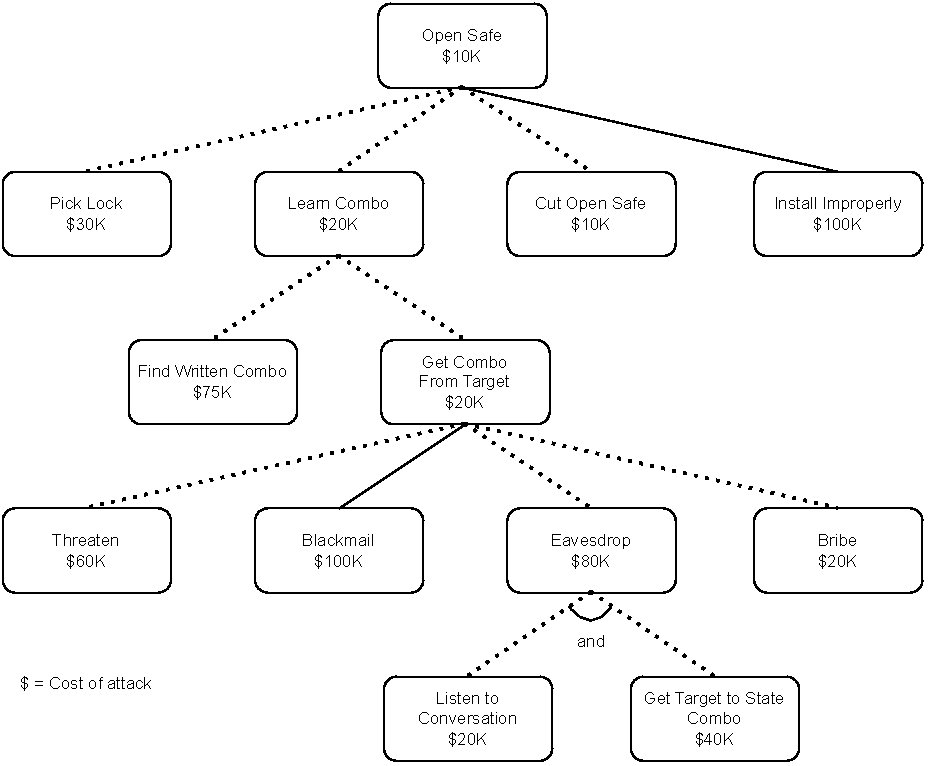
\includegraphics[width=0.8\linewidth]{figures/attack_graph.pdf}
  \caption[Illustration d'un graphe d'attaque décrivant un scénario de compromission d'un coffre-fort.]{Illustration d'un graphe d'attaque décrivant un scénario de compromission d'un coffre-fort. (adapté de~\cite{schneier1999modeling})~: L'objectif racine \emph{Open Safe} est décomposé en quatre voies principales : \emph{Pick Lock} (\$30K), \emph{Learn Combo} (\$20K), \emph{Cut Open Safe} (\$10K) et \emph{Install Improperly} (\$100K). Par défaut, un nœud est de type \textsc{OU} (réaliser l'un des enfants suffit) ;
    lorsqu'un \emph{and} est indiqué, il s'agit d'un \textsc{ET} (tous les enfants sont requis). Les montants représentent des coûts estimés : pour un \textsc{OU}, le coût du parent est le \emph{minimum} des coûts enfants ;
    pour un \textsc{ET}, les coûts \emph{s'additionnent}.}
  \label{fig:attack_graphs}
\end{figure}

\

\noindent
\textbf{Arbres attaque-défense}~: \quad Les arbres attaque-défense~\cite{BKordy2010} (arbres \acparen{AD}) sont des modèles graphiques représentant les objectifs de l'attaquant et les contre-mesures du défenseur sous la forme d'une structure arborescente. Les arbres \acn{AD} fournissent une représentation plus abstraite du système et des objectifs des attaquants, tandis que les graphes d'attaque fournissent une représentation plus concrète des composants du système et de leurs relations. Un exemple d'arbre \acn{AD} est illustré en \autoref{fig:bank_attack_defense_tree}. La racine de l'arbre \acn{AD} représente l'objectif ultime des cyberattaquants. Les sous-nœuds associés aux branches représentent les différentes stratégies d'attaque que l'attaquant pourrait utiliser pour atteindre son objectif. Ils peuvent être accompagnés de contre-mesures préventives ou réactives du défenseur (pare-feu, systèmes de détection d'intrusion, plans d'intervention en cas d'incident, etc.).
Les arbres \acn{AD} permettent d'identifier les points faibles de la défense d'un système~\cite{BKordy2010}.

\begin{figure}[h!]
  \centering
  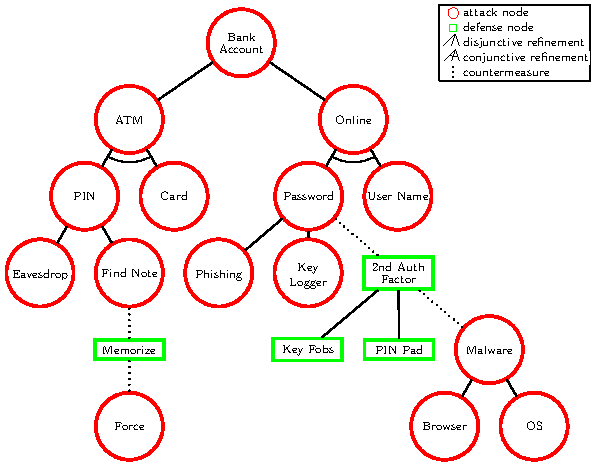
\includegraphics[width=\linewidth]{figures/adt.pdf}
  \caption[Illustration d'ADTree d'un scénario d'attaque sur un compte bancaire (tirée de~\cite{BKordy2010})]{Illustration d'ADTree décrivant un scénario d'attaque sur un compte bancaire (tirée de~\cite{BKordy2010})~: L'accès au compte peut être fait via un guichet automatique ou en ligne. Pour ce dernier cas, il est nécéssaire d'avoir un identifiant et un mot de passe obtenable par phishing ou un \textit{Key Logger}. Une contremesure à ces attaques est la double authentification construite avec une clé \textit{fob} ou un code pin.}
  \label{fig:bank_attack_defense_tree}
\end{figure}

\

\noindent
\textbf{Modélisation par réseaux de Petri}~: \quad Les réseaux de Petri pouvant être utilisés pour décrire des processus concurrents, certains travaux ont cherché à modéliser les attaquants et les défenseurs dans un système en réseau.
Les attaques extraites de bases de données peuvent être modélisées à l'aide de réseaux de Petri afin d'intégrer les cyberattaquants et les Cyberdéfenseurs, leurs stratégies et le coût de leurs actions, comme dans ~\cite{MPetty2022}. Les réseaux de Petri se révèlent également utiles pour modéliser les attaques par injection de langage de requête structuré afin d'inclure les stratégies des joueurs~\cite{JBland2020}.
Ils sont utilisés comme cadre pour évaluer et comparer plusieurs modèles d'attaque.
Dans ~\cite{SYamaguchi2020}, le logiciel malveillant \textit{Mirai} a aussi été exprimé sous la forme d'un modèle formel avec des réseaux de Petri, permettant de simuler un combat entre un agent défenseur et \textit{Mirai}.

\

\noindent
\textbf{Modèles de jeu}~: \quad Certains travaux ont proposé de modéliser les interactions entre les attaquants et les défenseurs dans un réseau comme des joueurs dans un jeu, où chaque joueur dispose d'un ensemble d'actions qu'il peut effectuer.
Parmi les travaux notables, citons~: Panfili et al.~\cite{MPanfili2018}, où un jeu à somme générale multi-agents opposant un attaquant à un défenseur est utilisé pour trouver un compromis optimal entre les actions de prévention et les coûts~; Attiah et al.~\cite{AAttiah2018}, où un cadre théorique de jeu dynamique est proposé pour analyser les interactions entre l'attaquant et le défenseur comme un jeu de sécurité non coopératif~; et Xiaolin et al.~\cite{CXiaolin2008}, qui utilisent des modèles de processus de Markov pour évaluer les risques dans les systèmes en réseau.

\noindent
Certaines approches fondées sur la théorie des jeux s'inscrivent dans le cadre des \textquote{jeux stochastiques partiellement observables} (\acn{POSG}) ou, plus précisément, dans celui des \textquote{processus de décision markoviens décentralisés partiellement observables} (\acn{Dec-POMDP}). Les \acn{POSG} et les \acn{Dec-POMDP} sont tous deux des cadres de modélisation mathématique des problèmes de prise de décision dans lesquels des agents interagissent entre eux et dans un environnement stochastique~\cite{beynier2010}. Dans un \acn{POSG}, un groupe d'agents interagit avec un environnement stochastique et partiellement observable. Chaque agent agit en fonction de ses propres observations et d'une politique locale. Les agents peuvent avoir des objectifs différents, car chaque agent a sa propre fonction de récompense et le jeu est généralement supposé être non coopératif~\cite{terry2020pettingzoo}. Dans un \acn{Dec-POMDP}, plusieurs agents peuvent avoir une fonction de récompense commune et peuvent coordonner leurs actions pour atteindre un objectif commun, notamment en étant capables de communiquer~\cite{bernstein2013}.



\subsection{Le modèle Dec-PODMP}\label{sec:dec-podmp}

Pour appliquer des techniques \acn{MARL}, il est nécéssaire de s'appuyer sur un cadre Markovien pour formaliser les observations, actions, récompense, etc. Nous nous basons sur le cadre du \acn{Dec-POMDP}~\cite{Oliehoek2016}. Les \acn{Dec-POMDP} permettent de modéliser la coordination décentralisée entre agents dans des contextes à observabilité partielle, ce qui les rend particulièrement adaptés à l'intégration de contraintes organisationnelles. Contrairement aux \acn{POSG}, le \acn{Dec-POMDP} utilise une fonction de récompense commune, favorisant ainsi la collaboration~\cite{Beynier2013}.

Un \acn{Dec-POMDP} $d \in D$ (avec $D$ l'ensemble des \acparen{Dec-POMDP}) est défini par un 7-uplet $d = (S,\{A_i\},T,R,\{\Omega_i\},O,\gamma)$ où~:
\begin{itemize}
  \item $S = \{s_1, ..., s_{|S|}\}$~: l'ensemble des états possibles.
  \item $A_i = \{a_1^i, ..., a_{|A_i|}^i\}$~: l'ensemble des actions possibles pour l'agent $i$.
  \item $T$ tel que $T(s,a,s') = \probP(s'|s,a)$~: la probabilité de transition conditionnelle entre états.
  \item $R: S \times A \times S \rightarrow \mathbb{R}$~: la fonction de récompense.
  \item $\Omega_i = \{o_1^i, ..., o_{|\Omega_i|}^i\}$~: l'ensemble des observations possibles pour l'agent $ag_i$.
  \item $O$ tel que $O(s',a,o) = \probP(o|s',a)$~: la probabilité conditionnelle d'observer $o$ depuis $s'$ après avoir effectué $a$.
  \item $\gamma \in [0,1]$~: le facteur d'actualisation qui décrit l'importance des récompenses futures par rapport aux récompenses immédiates (i.e spectre entre un comportement glouton et un comportement prévenant).
\end{itemize}

En considérant $m$ \textbf{équipes} (ou \textbf{groupes}) contenant chacune plusieurs agents parmi $\mathcal{A}$, nous reprenons le formalisme minimal nécessaire à la résolution d'un \acn{Dec-POMDP} pour une équipe donnée $i, 0 \leq i \leq m$, composée de $n$ agents~\cite{Beynier2013,Albrecht2024}~:

\begin{itemize}
  \item $\Pi$~: l'ensemble des politiques. Une \textbf{politique} $\pi \in \Pi, \pi~: \Omega \rightarrow A$ est une fonction déterministe qui associe à chaque observation une action. Elle représente la logique interne de l'agent.
  \item $\Pi_{joint}$~: l'ensemble des politiques conjointes. Une \textbf{politique conjointe} $\pi_{joint} \in \Pi_{joint}, \pi_{joint}~: \Omega^n \rightarrow A^n = \Pi^n$ associe une action à chaque agent en fonction de son observation, et peut être vue comme l'ensemble des politiques utilisées par les agents.
  \item $H$~: l'ensemble des historiques. Un \textbf{historique} sur $z \in \mathbb{N}$ étapes est un $z$-uplet $h = ((\omega_k, a_k) | k \leq z, \omega \in \Omega, a \in A)$.
  \item $H_{joint}$~: l'ensemble des historiques conjoints. Un \textbf{historique conjoint} sur $z$ étapes $h_{joint} \in H_{joint}, h_{joint} = \{h_1, h_2, ..., h_n\}$ est l'ensemble des historiques des agents.
  \item $U_{joint,i}(\langle \pi_{joint,i}, \pi_{joint,-i} \rangle): \Pi_{joint} \rightarrow \mathbb{R}$~: la \textbf{récompense cumulée espérée} pour l'équipe $i$ sur un horizon fini, avec $\pi_{joint,i}$ la politique conjointe de l'équipe $i$ et $\pi_{joint,-i}$ les politiques conjointes des autres équipes (considérées comme fixes).
  \item $BR_{joint,i}(\pi_{joint,i}) = \arg\max_{\pi_{joint,i}} U(\langle \pi_{joint,i}, \pi_{joint,-i} \rangle)$~: le \textbf{meilleur répondant} $\pi^*_{joint,i}$ tel qu'aucune modification de politique ne permettrait d'obtenir une récompense supérieure à $U^*_i = U_{joint,i}(\langle \pi^*_{joint,i}, \pi_{joint,-i} \rangle)$.
  \item $SR_{joint,i}(\pi_{joint,i}, s) = \{\pi_{joint,i} \mid U(\langle \pi_{joint,i}, \pi_{joint,-i} \rangle) \geq s\}$~: la \textbf{réponse suffisante}, c'est-à-dire l'ensemble des politiques conjointes atteignant au moins une récompense cumulée attendue $s \in \mathbb{R}, s \leq U^*_i$.
\end{itemize}

On appelle \textbf{résolution du \acn{Dec-POMDP}} la recherche d'une politique conjointe $\pi^j \in \Pi^j$ telle que $U_{joint,i}(\pi^j) \geq s$, atteignant une récompense cumulée espérée au moins égale à un seuil $s \in \mathbb{R}$.



\subsection{Les modèles de monde}

En \acn{RL}, et en particulier en contexte d'observabilité partielle, les \textbf{modèles du monde}~\cite{ha2018recurrent, hafner2020dream} ou \textit{World Models}\index{World Model} visent à apprendre des modèles internes approximant à la fois la dynamique de la fonction de transition et d'observation conjointement. Les \textit{World Models} permettent aux agents d'effectuer de la planification, d'améliorer l'efficacité échantillonnale, et de faciliter l'exploration sûre en permettant à l'agent de simuler des scénarios futurs. Cette approche appartient au paradigme du \acn{MBRL}~\cite{moerland2020model}, et se révèle particulièrement utile pour construire automatiquement des modèles de simulation à haute fidélité même en l'absence de représentation explicite de l'environnement.

Formellement, à chaque pas de temps $t$, on note $\omega_t \in \Omega$ l'observation courante, $a_t \in A$ l'action réalisée, et $\tilde{h}_{t-1} \in \mathcal{H}$ l'état caché récurrent résumant l'historique d'interaction jusqu'à $t-1$. Étant donné que les observations sont généralement de grande dimension (par exemple, des images ou des vecteurs d'état complexes), un encodeur $Enc: \Omega \rightarrow Z$ est appliqué pour projeter les observations dans un espace latent compact $Z$, avec $z_t = Enc(\omega_t)$, où $\dim(Z) \ll \dim(\Omega)$.

La structure temporelle principale est modélisée à l'aide d'un \textbf{Modèle Dynamique Latent Récurrent (\acparen{RLDM})}~\cite{hafner2020dream} $\mathcal{T}^{z} = f(g(h_{t-1}, z_t, a_t))$, qui prédit le prochain état latent $\hat{z}_{t+1}$ en mettant à jour l'état récurrent via $f$ et en appliquant une dynamique latente via $g$~:
\[
  \hspace{4cm}h_t = f(h_{t-1}, z_t, a_t), \quad \hat{z}_{t+1} = g(h_t)
\]
où $f(\cdot)$ correspond typiquement à un réseau de neurones récurrent \acn{RNN}\index{RNN} (par exemple un \acparen{LSTM}~\cite{hochreiter1997long}\index{LSTM}) appliqué à la concaténation de $h_{t-1}$, $z_t$ et $a_t$, et $g(\cdot)$ est une fonction (souvent implémentée par un \acparen{MLP}\index{MLP}) mappant l'état récurrent vers la représentation latente de la prochaine observation.

L'état latent prédit est ensuite décodé par $Dec: Z \rightarrow \Omega$ pour produire l'observation prédite $\hat{\omega}_{t+1} = Dec(\hat{z}_{t+1})$. L'ensemble du modèle est entraîné conjointement pour minimiser à la fois la \emph{perte de reconstruction} $\|\omega_{t+1} - \hat{\omega}_{t+1}\|$ dans l'espace d'observation, et éventuellement une \emph{perte de prédiction latente} pour stabiliser l'apprentissage de la dynamique latente.

L'état caché récurrent $\tilde{h}_t$ joue le rôle d'un résumé compact de l'historique complet d'interaction jusqu'au temps $t$, évitant ainsi d'avoir à stocker explicitement de longues séquences observation-action.

Par souci de concision, nous définissons la composition complète qui associe directement observation courante, action et état récurrent à l'observation prédite suivante sous la forme du \textbf{Modèle de Prédiction d'Observation} (\acparen{OPM})\index{Observation Prediction Model (OPM)}~:
\[
  \hspace{2cm}\mathcal{T}(h_{t-1}, \omega_t, a_t)~:= Dec(g(f(h_{t-1}, Enc(\omega_t), a_t))) = \hat{\omega}_{t+1}.
\]

\begin{figure}[h!]
  \centering
  \resizebox{\textwidth}{!}{%
    


\tikzset{every picture/.style={line width=0.75pt}} %set default line width to 0.75pt        

\begin{tikzpicture}[x=0.75pt,y=0.75pt,yscale=-1,xscale=1]
    %uncomment if require: \path (0,2102); %set diagram left start at 0, and has height of 2102

    %Straight Lines [id:da7945271061326031] 
    \draw    (100,1800) -- (111.5,1800) ;
    \draw [shift={(113.5,1800)}, rotate = 180] [color={rgb, 255:red, 0; green, 0; blue, 0 }  ][line width=0.75]    (6.56,-1.97) .. controls (4.17,-0.84) and (1.99,-0.18) .. (0,0) .. controls (1.99,0.18) and (4.17,0.84) .. (6.56,1.97)   ;
    %Straight Lines [id:da710289636295716] 
    \draw    (100,1835) -- (188,1834) -- (188,1820) ;
    \draw [shift={(188,1818)}, rotate = 90] [color={rgb, 255:red, 0; green, 0; blue, 0 }  ][line width=0.75]    (6.56,-1.97) .. controls (4.17,-0.84) and (1.99,-0.18) .. (0,0) .. controls (1.99,0.18) and (4.17,0.84) .. (6.56,1.97)   ;
    %Straight Lines [id:da9775676154282154] 
    \draw    (146.38,1800) -- (160,1800) ;
    \draw [shift={(162,1800)}, rotate = 180] [color={rgb, 255:red, 0; green, 0; blue, 0 }  ][line width=0.75]    (7.65,-2.3) .. controls (4.86,-0.97) and (2.31,-0.21) .. (0,0) .. controls (2.31,0.21) and (4.86,0.98) .. (7.65,2.3)   ;
    %Straight Lines [id:da789934339782699] 
    \draw    (100,1766) -- (122,1766) ;
    \draw [shift={(124,1766)}, rotate = 180] [color={rgb, 255:red, 0; green, 0; blue, 0 }  ][line width=0.75]    (6.56,-1.97) .. controls (4.17,-0.84) and (1.99,-0.18) .. (0,0) .. controls (1.99,0.18) and (4.17,0.84) .. (6.56,1.97)   ;
    %Shape: Trapezoid [id:dp2317709974845179] 
    \draw   (123.84,1754.74) -- (142.07,1760.21) -- (142.07,1771.42) -- (123.84,1776.88) -- cycle ;
    %Straight Lines [id:da7383754609221514] 
    \draw    (142,1766) -- (188,1766) -- (188,1780) ;
    \draw [shift={(188,1782)}, rotate = 270] [color={rgb, 255:red, 0; green, 0; blue, 0 }  ][line width=0.75]    (6.56,-1.97) .. controls (4.17,-0.84) and (1.99,-0.18) .. (0,0) .. controls (1.99,0.18) and (4.17,0.84) .. (6.56,1.97)   ;
    %Straight Lines [id:da49394763541143527] 
    \draw    (216,1800) -- (237.33,1799.94) ;
    \draw [shift={(239.33,1799.94)}, rotate = 179.85] [color={rgb, 255:red, 0; green, 0; blue, 0 }  ][line width=0.75]    (6.56,-1.97) .. controls (4.17,-0.84) and (1.99,-0.18) .. (0,0) .. controls (1.99,0.18) and (4.17,0.84) .. (6.56,1.97)   ;
    %Straight Lines [id:da8738633046359771] 
    \draw    (265.89,1800.03) -- (284.72,1800.03) ;
    \draw [shift={(286.72,1800.03)}, rotate = 180] [color={rgb, 255:red, 0; green, 0; blue, 0 }  ][line width=0.75]    (6.56,-1.97) .. controls (4.17,-0.84) and (1.99,-0.18) .. (0,0) .. controls (1.99,0.18) and (4.17,0.84) .. (6.56,1.97)   ;
    %Straight Lines [id:da3021616845453272] 
    \draw    (302,1800) -- (320.83,1800) ;
    \draw [shift={(322.83,1800)}, rotate = 180] [color={rgb, 255:red, 0; green, 0; blue, 0 }  ][line width=0.75]    (6.56,-1.97) .. controls (4.17,-0.84) and (1.99,-0.18) .. (0,0) .. controls (1.99,0.18) and (4.17,0.84) .. (6.56,1.97)   ;
    %Straight Lines [id:da8984410115217915] 
    \draw    (346,1800) -- (353.4,1800) -- (365.04,1800) ;
    \draw [shift={(367.04,1800)}, rotate = 180] [color={rgb, 255:red, 0; green, 0; blue, 0 }  ][line width=0.75]    (6.56,-1.97) .. controls (4.17,-0.84) and (1.99,-0.18) .. (0,0) .. controls (1.99,0.18) and (4.17,0.84) .. (6.56,1.97)   ;
    %Shape: Trapezoid [id:dp37639710819638017] 
    \draw   (423.61,1812) -- (405.38,1806.53) -- (405.38,1795.32) -- (423.61,1789.86) -- cycle ;
    %Straight Lines [id:da10289425963982124] 
    \draw    (384,1800) -- (403.04,1800) ;
    \draw [shift={(405.04,1800)}, rotate = 180] [color={rgb, 255:red, 0; green, 0; blue, 0 }  ][line width=0.75]    (6.56,-1.97) .. controls (4.17,-0.84) and (1.99,-0.18) .. (0,0) .. controls (1.99,0.18) and (4.17,0.84) .. (6.56,1.97)   ;
    %Straight Lines [id:da12692360321469986] 
    \draw    (424,1800) -- (443.04,1800) ;
    \draw [shift={(445.04,1800)}, rotate = 180] [color={rgb, 255:red, 0; green, 0; blue, 0 }  ][line width=0.75]    (6.56,-1.97) .. controls (4.17,-0.84) and (1.99,-0.18) .. (0,0) .. controls (1.99,0.18) and (4.17,0.84) .. (6.56,1.97)   ;
    %Shape: Trapezoid [id:dp27180057752038367] 
    \draw   (217.23,1670.74) -- (235.46,1676.21) -- (235.46,1687.42) -- (217.23,1692.88) -- cycle ;
    %Shape: Trapezoid [id:dp9437628483591106] 
    \draw   (309.61,1695) -- (291.38,1689.53) -- (291.38,1678.32) -- (309.61,1672.86) -- cycle ;
    %Straight Lines [id:da19635385567867214] 
    \draw    (310,1683) -- (328,1683) ;
    \draw [shift={(330,1683)}, rotate = 180] [color={rgb, 255:red, 0; green, 0; blue, 0 }  ][line width=0.75]    (6.56,-1.97) .. controls (4.17,-0.84) and (1.99,-0.18) .. (0,0) .. controls (1.99,0.18) and (4.17,0.84) .. (6.56,1.97)   ;
    %Straight Lines [id:da6136759960935583] 
    \draw    (196,1683) -- (214.83,1683) ;
    \draw [shift={(216.83,1683)}, rotate = 180] [color={rgb, 255:red, 0; green, 0; blue, 0 }  ][line width=0.75]    (6.56,-1.97) .. controls (4.17,-0.84) and (1.99,-0.18) .. (0,0) .. controls (1.99,0.18) and (4.17,0.84) .. (6.56,1.97)   ;
    %Straight Lines [id:da5198115307428596] 
    \draw    (236,1683) -- (255.04,1683) ;
    \draw [shift={(257.04,1683)}, rotate = 180] [color={rgb, 255:red, 0; green, 0; blue, 0 }  ][line width=0.75]    (6.56,-1.97) .. controls (4.17,-0.84) and (1.99,-0.18) .. (0,0) .. controls (1.99,0.18) and (4.17,0.84) .. (6.56,1.97)   ;
    %Straight Lines [id:da6362560665768464] 
    \draw    (270,1683) -- (289.04,1683) ;
    \draw [shift={(291.04,1683)}, rotate = 180] [color={rgb, 255:red, 0; green, 0; blue, 0 }  ][line width=0.75]    (6.56,-1.97) .. controls (4.17,-0.84) and (1.99,-0.18) .. (0,0) .. controls (1.99,0.18) and (4.17,0.84) .. (6.56,1.97)   ;
    %Shape: Rectangle [id:dp3864765488610862] 
    \draw  [color={rgb, 255:red, 74; green, 144; blue, 226 }  ,draw opacity=1 ][dash pattern={on 0.84pt off 2.51pt}] (70,1720) -- (475,1720) -- (475,1855) -- (70,1855) -- cycle ;
    %Shape: Rectangle [id:dp17767261593347572] 
    \draw  [color={rgb, 255:red, 65; green, 117; blue, 5 }  ,draw opacity=1 ][dash pattern={on 0.84pt off 2.51pt}] (175,1660) -- (355,1660) -- (355,1700) -- (175,1700) -- cycle ;
    %Shape: Polygon [id:ds8294746409292746] 
    \draw  [color={rgb, 255:red, 208; green, 2; blue, 27 }  ,draw opacity=1 ][dash pattern={on 0.84pt off 2.51pt}] (390,1845) -- (75,1845) -- (75,1780.92) -- (150,1780) -- (150,1750) -- (390,1750) -- cycle ;


    % Text Node
    \draw (333.5,1764.5) node  [color={rgb, 255:red, 208; green, 2; blue, 27 }  ,opacity=1 ] [align=left] {\footnotesize \textbf{\textit{RDLM}}};
    % Text Node
    \draw (317.5,1734.5) node  [color={rgb, 255:red, 74; green, 144; blue, 226 }  ,opacity=1 ] [align=left] {\footnotesize Modèle de prédiction d'observation (\textbf{\textit{OPM}})};
    % Text Node
    \draw (264.5,1645.5) node  [color={rgb, 255:red, 65; green, 117; blue, 5 }  ,opacity=1 ] [align=left] {{\footnotesize \textbf{Auto-encodeur}}};
    % Text Node
    \draw (189.5,1683) node  [font=\tiny] [align=left] {$\displaystyle \omega _{t}$};
    % Text Node
    \draw (340,1682) node  [font=\tiny] [align=left] {$\displaystyle \hat{\omega }_{t}$};
    % Text Node
    \draw (301.5,1679.5) node   [align=left] {{\tiny Dec}};
    % Text Node
    \draw (225.38,1676.5) node   [align=left] {{\tiny Enc}};
    % Text Node
    \draw (264.5,1684) node  [font=\tiny] [align=left] {$\displaystyle z_{t}$};
    % Text Node
    \draw (456.54,1799) node  [font=\tiny] [align=left] {$\displaystyle \hat{\omega }_{t+1}$};
    % Text Node
    \draw (415.5,1796.5) node   [align=left] {{\tiny Dec}};
    % Text Node
    \draw (375.5,1799) node  [font=\tiny] [align=left] {$\displaystyle z_{t+1}$};
    % Text Node
    \draw (132,1760.5) node   [align=left] {{\tiny Enc}};
    % Text Node
    \draw (295,1798) node  [font=\tiny] [align=left] {$\displaystyle \tilde{h}_{t}$};
    % Text Node
    \draw    (239.48,1779) -- (265.48,1779) -- (265.48,1817) -- (239.48,1817) -- cycle  ;
    \draw (252.48,1798) node  [font=\tiny] [align=left] {\begin{minipage}[lt]{14.99pt}\setlength\topsep{0pt}
            \begin{center}
                \phantom{X}\\\textit{RNN}
            \end{center}

        \end{minipage}};
    % Text Node
    \draw  [color={rgb, 255:red, 255; green, 255; blue, 255 }  ,draw opacity=1 ][fill={rgb, 255:red, 255; green, 255; blue, 255 }  ,fill opacity=1 ]  (157.5,1757) -- (174.5,1757) -- (174.5,1773) -- (157.5,1773) -- cycle  ;
    \draw (166,1765) node  [font=\tiny] [align=left] {$\displaystyle z_{t}$};
    % Text Node
    \draw    (162,1782) -- (216,1782) -- (216,1818) -- (162,1818) -- cycle  ;
    \draw (189,1800) node  [font=\tiny] [align=left] {\begin{minipage}[lt]{34pt}\setlength\topsep{0pt}
            \begin{center}
                \phantom{X}\\\textit{concatenate}
            \end{center}

        \end{minipage}};
    % Text Node
    \draw (91,1833) node  [font=\tiny] [align=left] {$\displaystyle \tilde{h}_{t-1}$};
    % Text Node
    \draw (91.5,1801) node  [font=\tiny] [align=left] {$\displaystyle a_{t}$};
    % Text Node
    \draw (91.5,1766) node  [font=\tiny] [align=left] {$\displaystyle \omega _{t}$};
    % Text Node
    \draw    (322.5,1792) -- (345.5,1792) -- (345.5,1807) -- (322.5,1807) -- cycle  ;
    \draw (334,1799.5) node  [font=\tiny] [align=left] {MLP};
    % Text Node
    \draw    (113,1788) -- (146,1788) -- (146,1813) -- (113,1813) -- cycle  ;
    \draw (129.5,1800.5) node  [font=\tiny] [align=left] {one-hot\\encode};


\end{tikzpicture}
  }
  \caption{Illustration de l'architecture d'un \textit{World Model} comprenant l'Auto-encodeur et l'OPM}
  \label{fig:single_agent_world_model}
\end{figure}

La \autoref{fig:single_agent_world_model} illustre l'architecture d'un \textit{World Model} comprenant l'Auto-encodeur et l'\acn{OPM}.

\textbf{Phase d'entraînement de l'auto-encodeur :} Un auto-encodeur, tel qu'un \acn{VAE}, est d'abord entraîné à encoder et décoder les observations en représentations latentes. L'objectif est de minimiser l'écart entre les observations réelles et les observations décodées.

\textbf{Initialisation et traitement des transitions :} Initialement, l'état caché récurrent $\tilde{h}_{t-1}$ est initialisé au vecteur nul. Pour chaque historique et chaque transition, un vecteur d'entrée est construit en concaténant trois éléments : la représentation de l'observation $z_t$, l'action $a_t$ (après encodage one-hot) et l'état caché récurrent $\tilde{h}_{t-1}$.

\textbf{Fonctionnement du \acn{RLDM} :} Ce vecteur d'entrée est traité par le \acn{RLDM} selon un processus en deux étapes. D'abord, il passe par le \acn{RNN} qui met à jour l'état caché récurrent avec les nouvelles transitions pour obtenir $\hat{h}_t$. Ensuite, ce vecteur est transmis à un \acn{MLP} qui détermine la représentation latente de l'observation suivante $\hat{z}_{t+1}$.

\textbf{Entraînement et prédiction :} Le \acn{RLDM} est entraîné à minimiser l'erreur quadratique entre l'observation prédite et l'observation réelle. Une fois l'entraînement terminé, une représentation latente d'observation prédite peut être décodée en une observation prédite $\omega_{t+1}$.

\section{Apprentissage par renforcement sous contraintes (TRN)}

L'apprentissage par renforcement sous contraintes vise à doter les agents de la capacité à optimiser leur comportement tout en respectant des exigences additionnelles, telles que la sûreté, l'équité ou des règles organisationnelles. Cette section présente les principaux cadres théoriques et techniques permettant d'intégrer explicitement ou implicitement des contraintes dans le processus d'apprentissage, en s'appuyant sur les extensions du \acn{RL} classique, les méthodes de Safe \acn{RL}, ainsi que les mécanismes de guidage organisationnel.

\subsection{Apprentissage par renforcement multi-agent}
% Rappeler les bases du \acn{MARL} et expliciter en utilisant le formalisme des \acn{Dec-POMDP} précédement défini

L'apprentissage par renforcement (\acparen{RL})\index{Apprentissage par renforcement (RL)} est un cadre formel dans lequel un agent apprend à agir dans un environnement inconnu en interagissant avec lui. À chaque étape, l'agent observe un état (ou une observation partielle), exécute une action, reçoit une récompense, et perçoit un nouvel état. L'objectif est de maximiser la récompense cumulée à long terme, généralement modélisée par une fonction de retour espéré.

Formellement, le problème est souvent représenté comme un processus de décision de Markov (\acparen{MDP}), défini par un quintuplet $\langle S, A, T, R, \gamma \rangle$, où~:
\begin{itemize}
  \item $S$ est l'ensemble des états~;
  \item $A$ est l'ensemble des actions possibles~;
  \item $T: S \times A \rightarrow \mathcal{P}(S)$ est la fonction de transition~;
  \item $R: S \times A \rightarrow \mathbb{R}$ est la fonction de récompense~;
  \item $\gamma \in [0,1]$ est le facteur d'actualisation.
\end{itemize}

L'agent apprend une politique $\pi~: S \rightarrow A$ (ou stochastique) qui maximise la somme des récompenses escomptées. Dans le cas partiellement observable (\acparen{POMDP}), les états sont inaccessibles, et l'agent agit à partir d'observations et d'un historique.


Dans le cas multi-agent, plusieurs agents interagissent simultanément avec l'environnement. Le problème devient plus complexe car~:
\begin{itemize}
  \item \textbf{L'environnement devient non-stationnaire}~: chaque agent modifie l'environnement et perturbe l'apprentissage des autres~;
  \item \textbf{L'exploration devient conjointe}~: les conséquences d'une action peuvent dépendre du comportement des autres~;
  \item \textbf{Le crédit d'attriobjectifion est difficile}~: relier une récompense à l'action d'un agent spécifique devient ambigu.
\end{itemize}

Le \acn{MARL}\index{Apprentissage par renforcement multi-agent (MARL)} traite de ces difficultés en adaptant les méthodes de \acn{RL} à ce contexte. Deux grandes approches peuvent être distinguées~:
\begin{itemize}
  \item \textbf{Apprentissage indépendant (Independent Learners)}~: chaque agent apprend sa politique en considérant les autres comme partie de l'environnement (simplifie la mise en œuvre mais génère de l'instabilité)~;
  \item \textbf{Apprentissage centralisé avec exécution décentralisée (\acparen{CTDE})}~: l'apprentissage est fait de manière coordonnée, avec accès à des informations globales (états, récompenses), mais les politiques finales doivent pouvoir s'exécuter de façon autonome.
\end{itemize}


Le \acn{MARL} a été appliqué avec succès dans plusieurs domaines~: coordination de robots, jeux coopératifs, gestion de trafic, systèmes énergétiques, etc. Dans le contexte de la Cyberdéfense, il offre un potentiel intéressant pour concevoir des politiques adaptatives capables de répondre à des menaces dynamiques et partiellement observées.

Cependant, plusieurs limites persistent~:
\begin{itemize}
  \item \textbf{La difficulté de convergence} dans des environnements complexes ou compétitifs~;
  \item \textbf{Le manque de garanties de sûreté ou de respect de contraintes}~;
  \item \textbf{Le peu d'explicabilité des politiques apprises}, souvent représentées par des réseaux de neurones~;
  \item \textbf{L'absence de structuration organisationnelle} explicite dans les architectures existantes.
\end{itemize}

Ces limitations motivent une intégration plus étroite entre méthodes d'apprentissage et modèles organisationnels, ce que nous explorerons dans les parties suivantes.



\subsection{Constrained MDPs, Safe RL et guidages implicites}

\noindent
L'un des principaux défis du \acn{RL} appliqué à des environnements critiques
comme la Cyberdéfense réside dans la capacité à garantir la sûreté des politiques apprises,
tout en maintenant l'adaptabilité propre à l'apprentissage connexionniste.
En effet, les méthodes classiques d'optimisation de politiques visent à maximiser une récompense cumulée,
sans tenir compte de contraintes additionnelles (sécurité, règles organisationnelles, équité, etc.).
Pour pallier cette limite, de nombreuses extensions ont été proposées, regroupées sous la bannière
du \textit{Safe RL} et des \textit{Constrained MDPs}.

\paragraph{Constrained Markov Decision Processes (CMDP).}
Un \textit{CMDP}~\cite{altman1999constrained} étend le cadre du \acn{MDP} classique en intégrant
un ensemble de coûts $C_i$ soumis à des bornes maximales $d_i$.
Un \acn{CMDP} est défini par un quintuplet
$\langle S, A, T, R, \{C_i\}, \gamma \rangle$,
où $(S,A,T,R,\gamma)$ correspond au \acn{MDP} standard, et où
chaque $C_i : S \times A \rightarrow \mathbb{R}$ représente une fonction de coût contrainte.
L'objectif devient alors~:
\[
  \hspace{1cm}\max_{\pi} \;\; \mathbb{E}\!\left[\sum_{t=0}^\infty \gamma^t R(s_t,a_t)\right]
  \quad \text{s.c.} \quad
  \mathbb{E}\!\left[\sum_{t=0}^\infty \gamma^t C_i(s_t,a_t)\right] \leq d_i, \;\; \forall i
\]
Ce formalisme généralise naturellement les problèmes de planification où certaines propriétés
(sûreté, consommation, risque) doivent être respectées en plus de la maximisation de la récompense.

\paragraph{Safe RL et optimisations contraintes.}
Dans la lignée des \acn{CMDP}, plusieurs méthodes ont été développées pour résoudre de manière pratique
des problèmes contraints. Parmi les plus notables~:
\begin{itemize}
  \item \textbf{Constrained Policy Optimization (\acn{CPO})}~\cite{achiam2017constrained},
        qui étend \acn{TRPO} en assurant,
        via une optimisation de type Lagrangien, que les contraintes ne soient
        pas violées au-delà d'un seuil fixé. Cette méthode fournit des garanties
        partielles de sûreté pendant l'entraînement.
  \item \textbf{Deep Constrained Q-Learning (\acn{DCQL})}~\cite{kalweit2020deep},
        qui adapte le Q-Learning profond aux environnements contraints
        en intégrant des multiplicateurs de Lagrange dans l'approximation
        de la fonction de valeur.
\end{itemize}

\paragraph{Guidages implicites.}
Au-delà des \acn{CMDP}, d'autres travaux proposent d'influencer indirectement
le comportement des agents par des mécanismes de guidage souples,
sans contraintes explicites~:
\begin{itemize}
  \item \textbf{Reward shaping}~\cite{ng1999policy}~: modification de la fonction
        de récompense afin d'inciter certains comportements (ex.~: coopération,
        respect de protocoles).
  \item \textbf{Shielding}~\cite{amodei2016concrete}~: filtrage a priori ou a posteriori
        des actions dangereuses grâce à un modèle de sûreté,
        empêchant l'agent d'exécuter des comportements interdits.
  \item \textbf{Feedback humain}~\cite{warnell2018deep}~: incorporation de corrections
        ou préférences fournies par un opérateur humain,
        permettant d'orienter l'apprentissage de manière interactive.
\end{itemize}

Les \acn{CMDP} et le Safe \acn{RL} apportent un premier niveau de garanties théoriques concernant le respect des contraintes, mais celles-ci restent généralement limitées à des contraintes locales (au niveau de l'action ou de la trajectoire) et de nature numérique. Les mécanismes de guidage implicites offrent une flexibilité appréciable, mais ne fournissent pas de garanties formelles. Par ailleurs, ces approches ne sont pas encore adaptées au contexte multi-agent, qui nécessiterait une extension du formalisme pour intégrer les interactions entre agents. Elles constituent néanmoins des bases importantes pour envisager l'intégration de contraintes organisationnelles plus expressives, que nous chercherons à articuler ultérieurement avec des modèles symboliques tels que $\mathcal{M}OISE^+$.

\subsection{Le modèle $\mathcal{M}OISE^+$}
% Modèles organisationnels (ex. MOISE+)
% Rôles, Missions, Permissions, Obligations (R-M-P-O)

\begin{figure}[h!]
  \centering
  


\tikzset{every picture/.style={line width=0.75pt}} %set default line width to 0.75pt        

\begin{tikzpicture}[x=0.75pt,y=0.75pt,yscale=-1,xscale=1]
%uncomment if require: \path (0,1656); %set diagram left start at 0, and has height of 1656

%Shape: Rectangle [id:dp6756844921493015] 
\draw  [fill={rgb, 255:red, 248; green, 231; blue, 28 }  ,fill opacity=1 ] (46,1204) -- (214,1204) -- (214,1424) -- (46,1424) -- cycle ;
%Shape: Rectangle [id:dp3759944257810566] 
\draw  [fill={rgb, 255:red, 80; green, 227; blue, 194 }  ,fill opacity=1 ] (390,1204) -- (556,1204) -- (556,1424) -- (390,1424) -- cycle ;
%Shape: Rectangle [id:dp28244406216006945] 
\draw  [fill={rgb, 255:red, 144; green, 19; blue, 254 }  ,fill opacity=1 ] (218,1234) -- (386,1234) -- (386,1338) -- (218,1338) -- cycle ;
%Shape: Rectangle [id:dp32232123359581766] 
\draw   (42,1176) -- (562,1176) -- (562,1428) -- (42,1428) -- cycle ;
%Shape: Rectangle [id:dp7605706269262755] 
\draw  [fill={rgb, 255:red, 74; green, 144; blue, 226 }  ,fill opacity=1 ] (396,1286) -- (550,1286) -- (550,1418) -- (396,1418) -- cycle ;
%Shape: Rectangle [id:dp33110985390647496] 
\draw   (52,1294) -- (210,1294) -- (210,1418) -- (52,1418) -- cycle ;
%Shape: Rectangle [id:dp8653560038381976] 
\draw  [fill={rgb, 255:red, 245; green, 166; blue, 35 }  ,fill opacity=1 ] (52,1294) -- (210,1294) -- (210,1418) -- (52,1418) -- cycle ;
%Straight Lines [id:da09781093164567278] 
\draw    (412,1350) -- (353.61,1307.18) ;
\draw [shift={(352,1306)}, rotate = 36.25] [color={rgb, 255:red, 0; green, 0; blue, 0 }  ][line width=0.75]    (10.93,-3.29) .. controls (6.95,-1.4) and (3.31,-0.3) .. (0,0) .. controls (3.31,0.3) and (6.95,1.4) .. (10.93,3.29)   ;
%Straight Lines [id:da3938396723807833] 
\draw    (122,1334) -- (264.04,1304.41) ;
\draw [shift={(266,1304)}, rotate = 168.23] [color={rgb, 255:red, 0; green, 0; blue, 0 }  ][line width=0.75]    (10.93,-3.29) .. controls (6.95,-1.4) and (3.31,-0.3) .. (0,0) .. controls (3.31,0.3) and (6.95,1.4) .. (10.93,3.29)   ;
%Shape: Rectangle [id:dp269311335478327] 
\draw  [color={rgb, 255:red, 208; green, 2; blue, 27 }  ,draw opacity=1 ][line width=1.5]  (66,1322) -- (122,1322) -- (122,1334) -- (66,1334) -- cycle ;
%Shape: Rectangle [id:dp7449860119164387] 
\draw  [color={rgb, 255:red, 208; green, 2; blue, 27 }  ,draw opacity=1 ][line width=1.5]  (412,1342) -- (488,1342) -- (488,1354) -- (412,1354) -- cycle ;


% Text Node
\draw (472.5,1237.41) node   [align=left] {\begin{minipage}[lt]{112.2pt}\setlength\topsep{0pt}
\begin{center}
\textbf{{\small Functional Specs.}}
\end{center}
{\small  - Social schemes $\displaystyle \mathcal{SCH}$}\\{\small  - Social preferences $\displaystyle \mathcal{SP}$}
\end{minipage}};
% Text Node
\draw (474,1355) node   [align=left] {\begin{minipage}[lt]{103.36pt}\setlength\topsep{0pt}
\begin{center}
\textbf{{\small Social Scheme.}}\\{\small \textbf{Specs. }$\displaystyle (\mathcal{SCH})$}
\end{center}
{\small  - Goals $\displaystyle \mathcal{G}$}\\{\small  - Missions $\displaystyle \mathcal{M}$}\\{\small  - Plans $\displaystyle \mathcal{P}$}\\{\small  - Mission to goals \ $\displaystyle mo$}\\\\{\small  ...}
\end{minipage}};
% Text Node
\draw (131,1356) node   [align=left] {\begin{minipage}[lt]{104.72pt}\setlength\topsep{0pt}
\begin{center}
{\small \textbf{Group Specs. }$\displaystyle (\mathcal{G} r)$}
\end{center}
{\small  - Roles $\displaystyle \mathcal{R}$}\\{\small  - Sub-groups $\displaystyle \mathcal{SG} \ \subset \mathcal{G} r$}\\{\small  - Links $\displaystyle \mathcal{L}$}\\{\small  - Compatibilities $\displaystyle \mathcal{C}$}\\\\{\small  ...}
\end{minipage}};
% Text Node
\draw (181,1177) node [anchor=north west][inner sep=0.75pt]   [align=left] {\begin{minipage}[lt]{162.41pt}\setlength\topsep{0pt}
\begin{center}
{\small \textbf{Organisational Specs. }$\displaystyle \mathcal{M}\boldsymbol{OISE^{+}}$($\displaystyle \mathbf{OS}$)}
\end{center}

\end{minipage}};
% Text Node
\draw (300,1269.09) node   [align=left] {\begin{minipage}[lt]{92.48pt}\setlength\topsep{0pt}
\begin{center}
\textbf{{\small Deontic Specs.}}
\end{center}
{\small  - Permissions $\displaystyle \mathcal{PER}$}\\{\small  - Obligations $\displaystyle \mathcal{OBL}$}
\end{minipage}};
% Text Node
\draw (130.5,1245.69) node   [align=left] {\begin{minipage}[lt]{112.2pt}\setlength\topsep{0pt}
\begin{center}
\textbf{{\small Structural Specs.}}
\end{center}
{\small  - Root-groups $\displaystyle \mathcal{G} r$}\\{\small  - Roles $\displaystyle \mathcal{R}_{ss}$}\\{\small  - Roles inheritance $\displaystyle \mathcal{IR}$}
\end{minipage}};


\end{tikzpicture}
  \caption{Vue synthétique du modèle $\mathcal{M}OISE^+$}
  \label{fig:moise_model}
\end{figure}

Le modèle $\mathcal{M}OISE^+$~\citep{Hubner2002}\index{MOISE+} fournit une description formelle avancée d'une organisation, notamment pour la description formelle des politiques des agents (via les plans). Il prend explicitement en compte les aspects sociaux entre agents, là où \acn{AGR} se concentre sur l'intégration de normes orientées conception. De plus, il propose une vision suffisamment détaillée de l'organisation pour être comprise selon différents points de vue. Une représentation visuelle des éléments formels de ce modèle est donné en \autoref{fig:moise_model}
En nous basant sur le formalisme de $\mathcal{M}OISE^+$~\citep{hubner2007moise}, nous ne détaillons ici que les éléments minimaux utilisés dans notre approche.

\

\noindent \textbf{\acn{OS}}~: \quad $\mathcal{OS} = \langle \mathcal{SS}, \mathcal{FS}, \mathcal{DS} \rangle$, l'ensemble des spécifications organisationnelles, où $\mathcal{SS}$ sont les \textbf{spécifications structurelles}, $\mathcal{FS}$ les \textbf{spécifications fonctionnelles}, et $\mathcal{DS}$ les \textbf{spécifications déontiques}.

\

\noindent \textbf{\acn{SS}}~: \quad $\mathcal{SS} = \langle \mathcal{R}, \mathcal{IR}, \mathcal{G} \rangle$, où~:

\begin{itemize}
  \item $\mathcal{R}_{ss}$~: l'ensemble des rôles (notés $\rho \in \mathcal{R}$)~;
  \item $\mathcal{IR}: \mathcal{R} \rightarrow \mathcal{R}$~: la relation d'héritage entre rôles ($\mathcal{IR}(\rho_1) = \rho_2$ signifie que $\rho_1$ hérite de $\rho_2$, noté aussi $\rho_1 \sqsubset \rho_2$)~;
  \item $\acn{RG} \subseteq \acn{GR}$~: l'ensemble des groupes racines, $\acn{GR} = \langle \mathcal{R}, \mathcal{SG}, \mathcal{L}^{intra}, \mathcal{L}^{inter}, \mathcal{C}^{intra}, \mathcal{C}^{inter}, np, ng \rangle$, l'ensemble des groupes, où~:
        \begin{itemize}
          \item $\mathcal{R} \subseteq \mathcal{R}_{ss}$~: l'ensemble des rôles non-abstraits~;
          \item $\mathcal{SG} \subseteq \mathcal{GR}$~: l'ensemble des sous-groupes~;
          \item $\mathcal{L} = \mathcal{R} \times \mathcal{R} \times \mathcal{TL}$~: l'ensemble des liens. Un lien est un triplet $(\rho_s,\rho_d,t) \in \mathcal{L}$ (aussi noté $link(\rho_s,\rho_d,t)$), où $\rho_s$ est le rôle source, $\rho_d$ le rôle destination, et $t \in \mathcal{TL}, \mathcal{TL} = \{acq, com, aut\}$ le type de lien~:
                \begin{itemize}
                  \item $t = acq$ (acquaintance)~: les agents jouant $\rho_s$ peuvent identifier les agents jouant $\rho_d$~;
                  \item $t = com$ (communication)~: les agents jouant $\rho_s$ peuvent communiquer avec ceux jouant $\rho_d$~;
                  \item $t = aut$ (authority)~: les agents jouant $\rho_s$ peuvent exercer une autorité sur ceux jouant $\rho_d$. Ce lien nécessite les liens d'acquaintance et de communication.
                \end{itemize}
          \item $\mathcal{L}^{intra} \subseteq \mathcal{L}$~: ensemble des liens intra-groupe~;
          \item $\mathcal{L}^{inter} \subseteq \mathcal{L}$~: ensemble des liens inter-groupe~;
          \item $\mathcal{C} = \mathcal{R} \times \mathcal{R}$~: l'ensemble des compatibilités. Une compatibilité est un couple $(\rho_a, \rho_b) \in \mathcal{C}$ (noté aussi $\rho_a \bowtie \rho_b$), signifiant qu'un agent jouant $\rho_a$ peut aussi jouer $\rho_b$~;
          \item $\mathcal{C}^{intra} \subseteq \mathcal{C}$~: ensemble des compatibilités intra-groupe~;
          \item $\mathcal{C}^{inter} \subseteq \mathcal{C}$~: ensemble des compatibilités inter-groupe~;
          \item $np: \mathcal{R} \rightarrow \mathbb{N} \times \mathbb{N}$~: relation donnant la cardinalité du nombre d'agents par rôle~;
          \item $ng: \mathcal{SG} \rightarrow \mathbb{N} \times \mathbb{N}$~: relation donnant la cardinalité de chaque sous-groupe.
        \end{itemize}
\end{itemize}

\medskip

\noindent \textbf{\acn{FS}}~: \quad $\mathcal{FS} = \langle \mathcal{SCH}, \mathcal{PO} \rangle$, où~:

\begin{itemize}
  \item $\mathcal{SCH} = \langle\mathcal{G}, \mathcal{M}, \mathcal{P}, mo, nm \rangle$~: l'ensemble des \textbf{schémas sociaux}, où~:
        \begin{itemize}
          \item $\mathcal{G}$~: l'ensemble des objectifs globaux~;
          \item $\mathcal{M}$~: l'ensemble des missions~;
          \item $\mathcal{P} = \langle \mathcal{G}, \{\mathcal{G}\}^s, OP, [0,1] \rangle, s \in \mathbb{N}^*$~: ensemble des plans qui définissent l'arbre des objectifs.
                Un plan $p \in \mathcal{P}$ est un 4-uplet $p = (g_f, \{g_i\}_{0 \leq i \leq s}, op, p)$, où $g_f \in \mathcal{G}$ est un objectif, les $g_i \in \mathcal{G}$ sont des sous-objectifs, $op \in OP = \{sequence, choice, parallel\}$ est un opérateur, et $p \in [0,1]$ est une probabilité de succès~:
                \begin{itemize}
                  \item $op = sequence$~: les $g_i$ doivent être atteints dans un ordre précis~;
                  \item $op = choice$~: un seul $g_i$ doit être atteint~;
                  \item $op = parallel$~: les $g_i$ peuvent être atteints en parallèle ou séquentiellement.
                \end{itemize}
          \item $mo: \mathcal{M} \rightarrow \mathbb{P}(\mathcal{G})$~: relation liant une mission à un ensemble de objectifs~;
          \item $nm: \mathcal{M} \rightarrow \mathbb{N} \times \mathbb{N}$~: cardinalité du nombre d'agents affectés à une mission.
        \end{itemize}
  \item $\mathcal{PO}: \mathcal{M} \times \mathcal{M}$~: ensemble des \textbf{ordres de préférence}. Un ordre de préférence est un couple $(m_1, m_2)$ (noté aussi $m_1 \prec m_2$) signifiant que si un agent peut s'engager à la fois sur $m_1$ et $m_2$, il aura une préférence sociale pour $m_1$.
\end{itemize}

\medskip

\noindent \textbf{\acn{DS}}~: \quad $\mathcal{DS} = \langle \mathcal{OBL}, \mathcal{PER} \rangle$, l'ensemble des spécifications déontiques, où~:

\begin{itemize}
  \item $\mathcal{TC}$~: ensemble des \textbf{contraintes temporelles}. Une contrainte $tc \in \mathcal{TC}$ indique les périodes pendant lesquelles une permission ou obligation est valide ($Any \in \mathcal{TC}$ signifie tout le temps)~;
  \item $\mathcal{OBL}: \mathcal{R} \times \mathcal{M} \times \mathcal{TC}$~: ensemble des \textbf{obligations}. Une obligation est un triplet $(\rho_a, m, tc)$ (aussi noté $obl(\rho_a, m, tc)$), signifiant qu'un agent jouant le rôle $\rho_a$ est obligé de s'engager dans la mission $m$ pendant la période spécifiée $tc$~;
  \item $\mathcal{PER}$~: ensemble des \textbf{permissions}. Une permission est un triplet $(\rho_a, m, tc)$ (aussi noté $per(\rho_a, m, tc)$), signifiant qu'un agent jouant le rôle $\rho_a$ est autorisé à s'engager dans la mission $m$ pendant $tc$.
\end{itemize}

\

\noindent Les spécifications organisationnelles appliquées aux agents sont les rôles et les objectifs (en tant que missions) à travers les permissions ou obligations. En effet, les autres spécifications structurelles comme les compatibilités ou les liens sont inhérentes aux rôles. De même, nous considérons que les objectifs, missions et leur association ($mo$) permettent de relier les autres spécifications fonctionnelles comme les plans, les cardinalités ou les préférences.
Par conséquent, nous considérons qu'il est suffisant de prendre en compte les rôles, les missions (objectifs et correspondance) et les permissions/obligations pour décrire l'essentiel de l'organisation d'un \acn{SMA}.


\section{Explicabilité et extraction organisationnelle (ANL)}

\noindent
L'explicabilité constitue un enjeu central dans la conception de \acplu{SMA}
appris par renforcement, en particulier dans des domaines critiques comme la Cyberdéfense.
Les politiques issues du \acn{MARL} sont souvent représentées par des réseaux de neurones
opaques, rendant difficile leur compréhension, leur validation et leur alignement
avec des spécifications organisationnelles.
L'objectif de cette section est de présenter les principales notions et techniques
mobilisées pour améliorer l'explicabilité et extraire des structures organisationnelles
émergentes à partir des comportements appris.

\subsection{Notion d'explicabilité}

\noindent
L'explicabilité peut être définie comme la capacité à fournir une description intelligible
des décisions ou comportements d'un système d'apprentissage automatique~\cite{doshivelez2017rigorous}.
Dans le cas du \acn{MARL}, deux niveaux d'explicabilité sont généralement distingués~:
\begin{itemize}
  \item \textbf{Explicabilité locale}~: comprendre les décisions d'un agent individuel
        à un instant donné, par exemple en reliant une action choisie
        à certaines observations ou caractéristiques de l'environnement.
  \item \textbf{Explicabilité globale}~: comprendre les structures collectives
        qui émergent au sein du \acn{SMA}, telles que la spécialisation
        des rôles, la coordination ou la réalisation d'objectifs collectifs.
\end{itemize}

Alors que l'explicabilité locale est bien couverte par les techniques classiques
d'explicabilité en apprentissage automatique (\acn{SHAP}, \acn{LIME}, attribution de gradient),
l'explicabilité globale est plus récente et reste un défi ouvert
\cite{poupart2025perspectives, milani2022maviper}.
Elle est pourtant essentielle pour analyser, comparer et certifier
les organisations implicites formées par apprentissage dans des contextes critiques.

\subsection{Méthodes post-hoc}

\noindent
Les méthodes \textit{post-hoc} visent à expliquer a posteriori des politiques déjà entraînées,
sans modifier leur processus d'apprentissage.
Elles permettent une meilleure compréhension des réseaux de neurones
au prix d'une explicabilité souvent locale ou partielle.

\paragraph{Attribution de caractéristiques.}
Des approches comme \acn{LRP}~\cite{bach2015lrp}
ou \acn{SHAP}~\cite{lundberg2017unified}
sont utilisées pour quantifier l'importance de chaque entrée
dans la prise de décision d'un agent.
Elles permettent de mettre en évidence les observations critiques
qui influencent une action donnée.

\paragraph{Patching et interventions.}
Grupen et al.~\cite{grupen2022concept} ont proposé des techniques
d'édition de modèles entraînés pour tester la sensibilité
des politiques apprises à des concepts spécifiques.
De même, l'utilisation d'approches dites de \textit{causal patching}
\cite{geiger2021causal} permet de comprendre la relation entre
représentations internes et comportements observés.

\paragraph{Attribution de concepts.}
Des travaux récents cherchent à relier directement des décisions
à des concepts humains interprétables,
par exemple via des réseaux neuronaux à base de concepts (\acn{CAV})
\cite{kim2018interpretability}
ou par attribution conceptuelle dans le \acn{MARL}
\cite{zabounidis2023concept}.
Ces approches ouvrent la voie à une explicabilité plus riche,
en reliant apprentissage connexionniste et représentations symboliques.

\subsection{Inférence organisationnelle}

\noindent
L'explicabilité globale suppose de dépasser l'analyse des décisions locales
pour reconstruire des structures organisationnelles implicites
(rôles, missions, relations de dépendance).
Plusieurs directions ont été explorées dans la littérature.

\paragraph{Clustering de trajectoires.}
L'analyse non supervisée des trajectoires d'agents permet d'identifier
des rôles ou missions émergents à partir de comportements récurrents.
Par exemple, Wang et al.~\cite{Wang2020} proposent l'approche \acn{ROMA}, où la spécialisation comportementale
des agents est favorisée par maximisation d'information mutuelle.
Plus largement, les techniques de clustering appliquées aux trajectoires
d'action/observation ouvrent la voie à une identification
automatique des rôles collectifs.

\paragraph{Approches bayésiennes et inférence de rôles.}
Certaines méthodes formalisent l'inférence organisationnelle
comme un problème probabiliste.
Yusuf et Baber~\cite{yusuf2020inferential} utilisent des modèles bayésiens
pour déduire les structures sociales implicites dans des environnements collaboratifs.
Des travaux plus anciens comme ceux de Berenji et Vengerov~\cite{berenji2000learning}
ont exploré l'apprentissage de rôles émergents à partir de la dynamique collective.

\paragraph{Vers un lien avec les modèles symboliques.}
L'un des défis actuels consiste à relier les structures émergentes
ainsi extraites à des modèles organisationnels explicites,
comme $\mathcal{M}OISE^+$~\cite{hubner2007using}.
Cette perspective ouvre la voie à une hybridation neurosymbolique,
où l'on pourrait rétro-inférer des spécifications organisationnelles
(rôles, missions, obligations) à partir des trajectoires observées,
puis les réinjecter pour guider de nouveaux apprentissages.
Des pistes récentes dans ce sens incluent les approches neurosymboliques
d'explicabilité en \acplu{SMA}~\cite{subramanian2024neurosymbolic}.

\

Les méthodes actuelles permettent une certaine transparence locale
et des inférences partielles sur les structures collectives,
mais aucun cadre unifié ne permet encore
d'extraire automatiquement des organisations complètes
et de les formaliser dans des modèles symboliques.
Ce verrou justifie la nécessité de contributions méthodologiques
pour développer des outils d'inférence organisationnelle
explicables, automatisés et exploitables dans des contextes opérationnels.

\section{Transfert simulation vers environnement réel et cohérence (TRF)}

\noindent
Un des défis majeurs du \acn{RL}, et en particulier du \acn{MARL}, réside dans l'écart
entre l'environnement simulé et l'environnement réel. Cet \textit{écart de réalité}
(\textit{reality gap}) limite la transférabilité des politiques apprises et
peut conduire à des comportements inefficaces, voire dangereux,
lors du déploiement opérationnel. La littérature propose plusieurs familles de méthodes
pour réduire cet écart et maintenir la cohérence entre simulation et réel~:
(i) l'adaptation de domaine (domain adaptation et \textit{Sim2Real}),
(ii) l'apprentissage par renforcement robuste,
(iii) l'adaptation en ligne, et
(iv) les approches de recalibrage manuel.

\subsection{Domain adaptation et Sim2Real}

\noindent
L'adaptation de domaine (\textit{domain adaptation}) consiste à rapprocher
les distributions de données issues de la simulation et du réel,
afin de rendre les politiques apprises transférables.
Deux grandes approches sont couramment employées~:

\begin{itemize}
  \item \textbf{Domain randomization}~\cite{tobin2017domain}~: l'idée est de
        randomiser massivement les paramètres de la simulation (textures, latences, topologies,
        probabilités de transition, etc.) afin que l'agent soit entraîné sur une distribution
        couvrant le réel comme un cas particulier. Formellement, si
        $p_\text{sim}(s'|s,a,\theta)$ désigne la dynamique simulée
        avec paramètres $\theta$, on échantillonne $\theta \sim \Theta$ pour
        maximiser la robustesse de la politique à la variabilité.
  \item \textbf{Domain invariance}~\cite{ganin2016domain}~: ici, on apprend
        des représentations latentes $z = f(o)$ des observations $o$
        de manière à rendre $z$ invariant au domaine
        (simulation vs réel). Cela s'écrit souvent comme une minimisation
        de divergence entre distributions latentes~:
        \[
          \hspace{3.5cm}\min_f \; D\big(p_\text{sim}(z), \; p_\text{real}(z)\big),
        \]
        où $D$ est une divergence statistique (\acn{KL}, \acn{MMD}, adversariale).
\end{itemize}

\noindent
Ces méthodes ont été utilisées avec succès en robotique~\cite{tobin2017domain, peng2018sim},
et commencent à être adaptées en cybersécurité~\cite{Standen2021}.
Elles permettent d'améliorer la fidélité et la transférabilité,
mais elles n'intègrent pas toujours de mécanismes d'adaptation en ligne.

\subsection{Robust Reinforcement Learning}

\noindent
Une seconde famille repose sur l'\textbf{apprentissage robuste}
(\textit{Robust RL}), qui vise à apprendre des politiques stables
face à l'incertitude des dynamiques de l'environnement~\cite{pinto2017robust}.
On suppose que les transitions appartiennent à un ensemble d'incertitude
$\mathcal{T}$ autour du modèle nominal $T$.
Le problème est alors formulé comme un jeu min-max~:
\[
  \hspace{3cm}\pi^* = \arg\max_\pi \; \min_{T \in \mathcal{T}}
  \; \mathbb{E}\!\left[\sum_{t=0}^\infty \gamma^t R(s_t,a_t) \;\middle|\; T, \pi\right]
\]
L'objectif est de maximiser le retour attendu
dans le pire cas de dynamique.
Cette approche fournit des garanties partielles de robustesse
au transfert simulation vers environnement réel,
au prix d'une politique souvent plus conservatrice.
Elle est utilisée notamment en robotique physique~\cite{pinto2017robust}
et dans des contextes critiques (énergie, cyber-physique).

\subsection{Adaptation en ligne}

\noindent
Les méthodes d'\textbf{adaptation en ligne} cherchent à
mettre à jour le modèle simulé ou la politique après déploiement,
à partir des retours observés.
Elles s'appuient sur des techniques d'\textit{online system identification}
et de boucles de rétroaction.

\begin{itemize}
  \item \textbf{Identification de systèmes en ligne}~: l'idée est d'estimer
        dynamiquement les paramètres du modèle $T_\theta$
        à partir des trajectoires réelles observées,
        via filtrage bayésien ou apprentissage incrémental~\cite{ljung1999system}.
  \item \textbf{PILCO}~\cite{deisenroth2011pilco}~: algorithme d'optimisation
        bayésienne basé sur des processus gaussiens,
        qui met à jour en ligne le modèle probabiliste de la dynamique
        pour planifier des politiques sûres.
  \item \textbf{World Models incrémentaux}~\cite{hafner2019learning}~:
        mise à jour continue des représentations latentes
        au fur et à mesure des interactions,
        permettant de maintenir la cohérence du jumeau numérique.
\end{itemize}

\noindent
Ces approches assurent une meilleure fidélité du modèle au réel,
mais augmentent la complexité computationnelle et nécessitent
des mécanismes de sûreté pour éviter des adaptations instables.

\subsection{Synchronisation manuelle}

\noindent
Enfin, une approche plus pragmatique et répandue consiste à
\textbf{recalibrer manuellement} la simulation
à intervalles réguliers à partir de données réelles.
C'est le cas de plusieurs simulateurs de Cyberdéfense tels que
\acn{CybORG}~\cite{Standen2021} ou
\acn{CyberBattleSim}~\cite{cyberbattlesim},
où les scénarios, topologies et vulnérabilités sont mis à jour
manuellement par des experts.
Cette approche est simple à mettre en œuvre,
mais elle est peu adaptée à des environnements très dynamiques,
et ne garantit pas la cohérence continue entre simulation et réalité.

\section{Bilan}
\noindent
En résumé, plusieurs stratégies complémentaires existent
pour réduire l'écart entre simulation et réel.
Les approches \textit{Sim2Real} (domain randomization, invariance)
couvrent le transfert initial,
le \textit{Robust RL} fournit des garanties partielles en environnement incertain,
l'adaptation en ligne permet de maintenir la cohérence dans la durée,
et le recalibrage manuel reste la pratique dominante en cybersécurité.
Cependant, aucun cadre unifié n'assure simultanément
la mise à jour conjointe du modèle simulé et des politiques déployées,
ce qui constitue un verrou scientifique majeur pour le transfert sûr
des politiques de \acn{SMA} dans des environnements critiques.

\clearpage
\thispagestyle{empty}
\null
\newpage


\chapter*{Conclusion}
\addcontentsline{toc}{chapter}{\textbf{Conclusion}}

\noindent
Cette deuxième partie a posé les fondations théoriques et critiques nécessaires à l'élaboration de notre méthode de conception. En s'appuyant sur les enjeux identifiés dans la \autoref{part:contexte}, elle a permis de clarifier les concepts mobilisés, d'identifier les verrous qui justifient la nécessité d'une nouvelle approche.

\medskip

\noindent
Le \autoref{chap:concepts} a introduit les trois piliers conceptuels sur lesquels s'appuie notre démarche~: (1) les modèles organisationnels, en particulier \textit{$\mathcal{M}OISE^+$}, qui offrent une structuration explicite du \acn{SMA}~; (2) Le \acn{MARL}, qui permet une acquisition autonome de politiques dans des environnements complexes~; et (3) les \textit{World Models}, qui fournissent un moyen de simuler un environnement à partir de données, ouvrant la voie à une exploration sécurisée et accélérée.

\noindent
Le \autoref{chap:verrous} a prolongé cette analyse en examinant les limites de l'état de l'art face aux exigences soulevées par notre question. Chaque hypothèse de recherche (\textbf{H-MOD} à \textbf{H-TRF}) a été replacée dans son contexte scientifique, discutée à la lumière des travaux existants, et reliée à un verrou spécifique~:
\begin{itemize}
  \item la difficulté à représenter le problème de conception dans un cadre intégrant l'environnement réel (\textbf{H-TRF})~;
  \item l'absence de \textit{World Models} ou framework de modélisation d'un environnement de Cyberdéfense adaptés au contexte multi-agent (\textbf{H-MOD})~;
  \item le manque d'intégration de contraintes organisationnelles dans l'apprentissage (\textbf{H-TRN})~;
  \item l'impossibilité d'analyser les comportements appris à l'échelle organisationnelle (\textbf{H-ANL}).
\end{itemize}

\medskip

\noindent
Ces constats convergent vers un besoin commun~: celui d'une méthode unifiée, capable d'orchestrer l'ensemble du processus de conception (de la modélisation de l'environnement à l'analyse des comportements) en intégrant apprentissage et organisation dans une boucle cohérente. C'est précisément l'objectif de la méthode \acn{MAMAD}, que nous introduisons dans la partie suivante.
